%%%%%%%%%%%%%%%%%%%%%%%%%%%%%%%%%%%%%%%%%%%%%%%%%%%%%%%%%%%% 
% This is the official template for theses and seminar papers from the Chair for Information Systems for Sustainable Society (IS3) at the University of Cologne

%
%PREAMBLE
%%%%%%%%%%%%%%%%%%%%%%%%%%%%%%%%%%%%%%%%%%%%%%%%%%%%%%%%%%%%%

\documentclass[a4paper, oneside, 11pt]{report}
\usepackage[utf8]{inputenc}
\usepackage[T1]{fontenc}
\usepackage{graphicx}
\usepackage{hyperref}
\usepackage{caption}
\usepackage{appendix}
\usepackage{amsfonts}
\usepackage{mathtools}
\usepackage{amsmath}
\usepackage{amsthm}
\usepackage{listings}

\newtheorem*{remark}{Remark}

% set margins for double-sided printing
\usepackage[left=3cm, right=3cm, top=2.5cm, bottom=2.5cm, bindingoffset=0cm, head=15pt]{geometry} 
\usepackage{setspace}
%\onehalfspacing

% set APA citation style
%\usepackage{apacite}
\usepackage[numbib,notlof,notlot,nottoc]{tocbibind}
\pagenumbering{gobble}


%%%%%%%%%%%%%%%%%%%%%%%%%%%%%%%%%%%%%%%%%%%%%%%%%%%%%%%%%%%%%
%THESIS Parameters 
%%%%%%%%%%%%%%%%%%%%%%%%%%%%%%%%%%%%%%%%%%%%%%%%%%%%%%%%%%%%%

\title{An Investigation of Decoupling Single Element Solutions from the Mesh in the Finite Element Method on Nvidia GPUs}

\newcommand{\thesisdate}{\today}
\newcommand{\thesisauthor}{Alex Keating} %input name
\newcommand{\studentID}{17307230} %input student ID
\newcommand{\thesistype}{MSc. High Performance Computing} % Set either to Bachelor or Master
\newcommand{\supervisor}{Jose Refojo \& Prof. Kirk Soodhalter}
\newcommand{\cosupervisor}{}

%%%%%%%%%%%%%%%%%%%%%%%%%%%%%%%%%%%%%%%%%%%%%%%%%%%%%%%%%%%%%
%DOCUMENT
%%%%%%%%%%%%%%%%%%%%%%%%%%%%%%%%%%%%%%%%%%%%%%%%%%%%%%%%%%%%%

\begin{document}

%%%%%%%%%%%%%%%%%%%%%%%%%%%%%%%%%%%%%%%%%%%%%%%%%%%%%%%%%%%%%
%TITLE PAGE (Pre-defined, just change parameters above)
%%%%%%%%%%%%%%%%%%%%%%%%%%%%%%%%%%%%%%%%%%%%%%%%%%%%%%%%%%%%%
%%%%%%%%%%%%%%%%%%%%%%%%%%%%%%%%%%%%%%%%%%%%%%%%%%%%%%%%%%%%%
%TITLE PAGE
%%%%%%%%%%%%%%%%%%%%%%%%%%%%%%%%%%%%%%%%%%%%%%%%%%%%%%%%%%%%%
\makeatletter
\begin{titlepage}
    \begin{center}
        \vspace*{1cm}

        \huge
        \textbf{\@title}

        \vspace{1cm}
        \LARGE
        \thesistype{}
        
        %\vspace{1cm}
		\vfill

        \begin{figure}[htbp]
             \centering
             
\includegraphics[width=0.8\linewidth]{./Figures/logo2}
        \end{figure}
		
		\vfill
        %\vspace{1cm}

        \Large
        \textbf{Author}: \thesisauthor{} \\
        \textbf{Student ID}: \studentID{}\\
        \textbf{Supervisor}: \supervisor{}\\
        %\large
        %\textbf{Co-Supervisor}: \cosupervisor{}

        \vspace{1.5cm}
        School of Mathematics\\
        Faculty of Engineering, Mathematics and Science\\
        Trinity College Dublin, University of Dublin\\

        \vspace{1cm}
        \@date

    \end{center}
\end{titlepage}
\makeatother


%%%%%%%%%%%%%%%%%%%%%%%%%%%%%%%%%%%%%%%%%%%%%%%%%%%%%%%%%%%%%
%SOOA
%%%%%%%%%%%%%%%%%%%%%%%%%%%%%%%%%%%%%%%%%%%%%%%%%%%%%%%%%%%%%
\clearpage
\thispagestyle{empty}
\section*{Declaration}
\label{sec:SOOA}

\vspace{1cm}

I have read and I understand the plagiarism provisions in the General 
Regulations of the University Calendar for the current year, found at 
\url{http://www.tcd.ie/calendar}.

\vspace{1cm}

\noindent
I have completed the Online Tutorial in avoiding plagiarism 'Ready, Steady, 
Write', located at \url{http://tcd‐ie.libguides.com/plagiarism/ready‐steady‐write}.

\vspace{1cm}
\noindent
\textbf{\thesisauthor{}} 

\vspace{0.5cm}
\noindent
\today



%%%%%%%%%%%%%%%%%%%%%%%%%%%%%%%%%%%%%%%%%%%%%%%%%%%%%%%%%%%%%
%ACKNOWLEDGEMENTS
\clearpage
\thispagestyle{empty}
\section*{Acknowledgements}
\label{sec:ack}

\vspace{1.0cm}

\begin{small}
I would like to use this space to firstly thank my supervisors Jose Refojo and Kirk Soodhalter; Jose for all his help, involving anything everything CUDA related and for going out of his way to come in on weekends to assist in doing my profiling. Kirk for all his help and guidance with the mathematics behind the finite element method and for always making himself available even when on different time-zones. I would like to thank both my parents, my grandmother and my sister, for all their help and support, and without whom, my completion of this degree would not have been possible. I would like to thank my lecturers and my classmates for their assistance throughout the year. Finally, I would like to give a thank you to all my family, friends, and in particular my housemates, and anyone else who supported me and listened to my complaints through what was a tough but enjoyable year . Thank you all.
\end{small}


%%%%%%%%%%%%%%%%%%%%%%%%%%%%%%%%%%%%%%%%%%%%%%%%%%%%%%%%%%%%%
%ABSTRACT
%%%%%%%%%%%%%%%%%%%%%%%%%%%%%%%%%%%%%%%%%%%%%%%%%%%%%%%%%%%%%
\clearpage
\clearpage
\thispagestyle{empty}
\section*{Abstract}

\vspace{1.0cm}

\begin{small}
In this thesis, an investigation was completed into parallelising the finite element method (FEM) on Nvidia GPUs. Naive CPU and basic GPU implementations were coded using C++11 and CUDA. The GPU implementation was parallelised by partitioning up the mesh's cells across the threads on the GPU and assembling the global stiffness matrix in parallel. Both CPU and GPU variants used pre-existing solvers (Intel MKL and cuSOVLER) to solve the final linear system. The results were tested against a simplistic rectangular mesh domain for the Laplace equation. These were tested and profiled, and the results showed large speed-ups to the point of assembly, but the linear systems solvers were outperformed by Intel's sparse solver. The linear system was also deemed to be the dominant kernel by a long stretch.

A novel finite element method single-element solution (FEMSES) approach was also implemented. This involved decoupling the local solutions from the entire mesh, and applying a Jacobi relaxation scheme to find local solutions to the element matrices. These were then assembled into a global solution estimate and iterated until convergence. This avoided the need to assembly the global stiffness matrix, thereby supposedly taking a large bottleneck out of the FEM and improving on its level of parallelism. FEMSES was tested and its timings compared back to that of the naive GPU approach on two different GPU architectures. The speed-ups seen were not matching of that drawn from FEMSES's original literature.

All related software to the report is located at \url{https://github.com/keatina3/FEMSES_project} .

\end{small}


%%%%%%%%%%%%%%%%%%%%%%%%%%%%%%%%%%%%%%%%%%%%%%%%%%%%%%%%%%%%%
%TOC,TOF,TOT
%%%%%%%%%%%%%%%%%%%%%%%%%%%%%%%%%%%%%%%%%%%%%%%%%%%%%%%%%%%%%
\pagenumbering{Roman}
\tableofcontents
\clearpage
\addcontentsline{toc}{chapter}{\listfigurename}
\listoffigures
\clearpage
\addcontentsline{toc}{chapter}{\listtablename}
\listoftables
\clearpage
\pagenumbering{arabic}


%%%%%%%%%%%%%%%%%%%%%%%%%%%%%%%%%%%%%%%%%%%%%%%%%%%%%%%%%%%%%
%MAIN PART
%%%%%%%%%%%%%%%%%%%%%%%%%%%%%%%%%%%%%%%%%%%%%%%%%%%%%%%%%%%%%


\clearpage
\chapter{Introduction}

Nowadays, with the advent of modern computing, there has been a huge push towards taking advantage of these resources. In the scientific world, there is a constant drive towards building optimised libraries for performing operations, spanning areas such as, basic linear algebra [CITE], fast Fourier transformations [CITE] or genetic algorithms for machine learning [CITE]. All of these libraries have been written with the intentions of exhausting as much processing power, memory and parallelisation as possible. These libraries are available across all kinds of architectures, Intel's MKL for example built for Intel CPUs, Nvidia's CUDA SDK written for their own GPUs or MAGMA, a 3rd party library written for heterogeneous architectures. These advancements in scientific computing have not come from nowhere, but rather are becoming duly necessary as most modern problems in science become impossible to solve without taking advantage of modern computing resources. A clear example of this was seen last year when the first image of a black hole was rendered, using a novel image cleaning machine learning algorithm and 5 petabytes of data - clearly something that cannot be done without some form of distributed memory architecture.

Nvidia have been among the leaders of this charge from both a hardware and software point...

The need for taking advantage of parallelism in modern science now clear, one problem that crops up in a vast array of areas is solving partial differential equations, or PDEs. These are relationships between variables and their partial derivatives and can be seen in areas such as fluid dynamics with the Navier-Stokes equations, in finance with the Black-Scholes equation or even in engineering when modelling stress of a structure - an important one for the topic at hand in this paper. Unfortunately, while analytic solutions exist for theoretical problems of this nature, studied in undergraduate courses, in the real world most of these PDEs are not of this convenient solvable nature and thus require numerical methods to solve. There are many variants of numerical methods which one can use to solve PDEs, some more simple than others, such as the finite difference method which decomposes the domain into a simple grid and approximates the derivatives, and some more complex but robust, like meshfree methods which create a collection of Voronoi cells on the domain instead of a basic grid - allowing for more complex structures. Certain methods land somewhere in a middle ground of both complexity and adaptability such as the finite volume method and the finite element method - the later of which will form the basis of this study.

The finite element method [CITE STRANG] is a numerical method developed originally for use in engineering for modelling stress on structures and has since quickly expanded to use in all branches of science such as electrostatics, something and something. Its engineering foundations will become clear throughout the paper as much of the terminology has remained unchanged. This paper will investigate current approaches to applying the finite element method on Nvidia GPUs and attempt at isolating and pinpointing certain bottlenecks for parallelism upon which may be improved. The importance of this is clear, as PDE-related problems get larger and more complex, the  need for more computing power is evident to get approximate solutions in reasonable amounts of time.

SECTION ON EXISTING FEM LIBRARIES 

\section{Preliminaries}
Maybe ???

\clearpage
\chapter{Finite Element Method}

This paper focuses its mathematics on implementing the finite element method to solve PDEs. This chapter will go through the necessary mathematics behind each of the steps behind the finite element method such as variational calculus, approximation theory and the finite elements themselves. The chapter also goes through the actual approach itself, alongside the worked example for the case of this study of the Laplace equation.

\section{General Problem}

Before the nuts and bolts of the finite element method are discussed, let us first consider an $n$-dimensional, general n\textsuperscript{th} order PDE of the form,
\begin{equation}
	f\left(\mathbf{x}; u(\mathbf{x}), \frac{\partial u}{\partial x_1},\dots, \frac{\partial u}{\partial x_n}; \frac{\partial^2 u}{\partial x_1 \partial x_1},\dots, \frac{\partial^2 u}{\partial x_1 \partial x_n}; \dots\right) = 0,
\end{equation}
where $\mathbf{x} = \{x_1,x_2,\dots,x_n\}$.
For a case of a 2-dimensional, 2\textsuperscript{nd} order PDE, we end up with the operator,
\begin{equation}
	\mathcal{L} = a \frac{\partial^2 u}{\partial x^2} + b \frac{\partial^2 u}{\partial x \partial y} + c \frac{\partial^2 u}{\partial y^2} + F\left(x,y; u; \frac{\partial u}{\partial x}, \frac{\partial u}{\partial y}\right).
\end{equation}
This can be used, applied to a function to leave a PDE,
\begin{equation}
	\mathcal{L}u = 0,
\end{equation}
which is going to be our entire basis for this study - attempting to approximate the function $u$. This problem can then be bounded by three types of non-homogeneous boundary conditions in order to be properly posed and have a unique/non-trivial solution:
\begin{enumerate}
	\item Dirichlet condition: $u=g(s)$.
	\item Neumann condition: $\frac{\partial u}{\partial \mathbf{n}} = h(s)$.
	\item Robin condition: $\frac{\partial u}{\partial \mathbf{n}} + \sigma(s)u = k(s)$,
\end{enumerate}
where $s$ is he arc length of the boundary $C$ and $\mathbf{n}$ is a vector, externally normal to $C$. How these conditions are imposed and handled will be seen later in the report.

\section{Approximation Theory}

Suppose there exists some function $u(x)$ that we wish to approximate. The most common way to is to estimate the value of the function using a collection of \textit{basis functions} $\psi_i(x)$, and unknown coefficients, $c_i$, giving,
\begin{equation}
	u(x) \approx \sum_{i=0}^N c_i\psi_i(x).
\end{equation}
There are a collection of ways to construct your basis functions and obtain solutions to the approximation (REFERENCE EQ) and this paper looks at three in particular:
\begin{itemize}
	\item least squares.
	\item Galerkin.
	\item weighted residuals.
\end{itemize}
There are other methods of approximation such as collocation and regression but they are not discussed here. Before these approaches are explained, two things must first be defined. Firstly, consider a function space $V$ defined by the span of set of basis functions,
\begin{equation}
	V = \text{span}\{\psi_0,\dots,\psi_N\},
\end{equation}
then it can be said the any function $u\in V$ can be written as a linear combination of the basis functions,
	\begin{equation}
		u(x) = \sum_i c_i \psi_i. 
	\end{equation}
Consider now, functions $f,g$ - the squared norm or inner-product of these two functions is defined as,
\begin{equation}
	\langle f,g\rangle = \int f(x)g(x)dx
\end{equation}
\subsection{Least Squares}
Suppose we are given a function $f(x)$ which needs to be approximated by a function $u(x)$ $\in V$ as defined above. The most obvious way to approximate this function would be to minimise the differential between the two, $f-u$. Subbing this into the inner product we are left with,
\begin{align}
	e &= \langle f-u, f-u\rangle = \langle f-\sum_i c_i \psi_i,f-\sum_i c_i \psi_i\rangle,\\
	e &= \langle f,f\rangle - 2~\sum_i c_i\langle f,\psi_i\rangle + \sum_{i,j} c_i c_j \langle\psi_i, \psi_j\rangle. 
\end{align}
Of course, now as is well known from optimisation, to minimise this residual function, its derivative must be taken at each of the $N$ points, $\frac{\partial e}{\partial c_i}$. Evaluating and setting $\frac{\partial e}{\partial c_i}$, results in the equation,
\begin{equation}
	- \langle f,\psi_i\rangle + \sum_j c_j\langle \psi_i, \psi_j\rangle = 0,\quad i \in \{0,\dots,N\},
\end{equation}
which can equally be written as,
\begin{equation}
	\sum_j A_{i,j}c_j = b_i,
\end{equation}
where,
\begin{align}
	A_{i,j} &= \langle \psi_i, \psi_j\rangle,\\
	b_i &= \langle f, \psi_i \rangle.
\end{align}
Now there is a system of linear equations which can be solved by usual means to obtain the approximation $u(x)$ of the function $f(x)$. Mathematically, it is equivalent to say that the method of least squares utilises the inner-product of the residuals, and solves by minimising it,
\begin{equation}
	\min_{c_0,\dots,c_N} \langle e, e\rangle,
\end{equation}
giving the system of $N+1$ equations,
\begin{equation}
	\left\langle e, \frac{\partial e}{\partial c_i}\right\rangle = 0, \quad i\in\{1,\dots,N\}.
\end{equation}

\subsection{Galerkin}

	In the previous subsection, it was seen that the least squares method operates by minimising the error term between the two functions, or alternatively, forcing the error to be orthogonal to the function space $V$. However, in reality, we do not actually know the true error as $f$ is not explicitly known and so instead a residual $R$ is used. Take for example, Eq.~(REFERENCE HERE), if we sub in an approximation $\hat{u} = \sum_i c_i \psi_i$, we get,
\begin{equation}
	R = \mathcal{L}\left(\sum_i c_i \psi_i\right) \neq 0.
\end{equation}
Now, the residual $R$ can be made orthogonal to the space $V$ by imposing,
\begin{equation}
	\langle R, v \rangle=0, \forall v \in V,
\end{equation}
and since any function in $V$ can be approximated using (REFERENCE), it can be said that,
\begin{equation}
	\langle R, \psi_i \rangle=0,\quad i\in\{1,\dots,N\},
\end{equation}
thus leaving another system of linear equations to solve. This is also known as projecting $R$ onto $V$.

\subsection{Weighted Residuals}

The method of weighted residuals is a relatively simple generalisation of the standard Galerkin method. Rather than imposing that the residual is orthogonal to the space $V$ known as the trial space, it is chosen to be orthogonal to some other space $W$, also known as the test space. This leaves the equation,
\begin{equation}
	\langle R, v \rangle=0, \forall v \in W,
\end{equation},
where,
\begin{equation}
	W = \text{span}\{w_0,\dots,w_n\}
\end{equation}
and so this leaves,
\begin{equation}
	\langle R, w_i \rangle=0,\quad i\in\{1,\dots,N\},
\end{equation}
again, leaving a system of $N+1$ linear equations.

\section{Variational Calculus}

\subsection{Weak Formulation}
As it should be clear by now, the overall aim of the finite element method is the minimise a residual in order to get an approximation of the function $u$ as seen in (REFERENCE). What may not seem immediately obvious at a first glance, but an important thing to factor in, (REFERENCE) is not how the PDE problem is usually posed when trying to apply FEM. In fact, usually, the problem is posed in its \textit{weak formulation}. The weak form of this equation is one which contains at most first-order derivative, as opposed to its strong form containing second-order derivatives. Usually, if only approximating a function, this issue wouldn't crop up. However, when dealing with calculus of variations, one must remember that boundary conditions must be imposed and reducing the order of derivatives weakens the demands on the test and trial functions, allowing them to not need be continuous in their second derivative.

Take for example a general PDE defined,
\begin{align}
	\mathbf{v}\cdot\nabla u + \beta u &= \nabla\cdot(\alpha\nabla u) + f,\quad  \mathbf{x} \in \Omega \\
	u &= u_D,\quad \mathbf{x} \in \Gamma_D\\
	-\alpha\frac{\partial u}{\partial \mathbf{n}} &= g,\quad \mathbf{x} \in \Gamma_N,
\end{align}
multiplying this by a test function $v$ and getting the inner product over the domain $\Omega$, just like was seen in the method of weighted residuals leaves the equation,
\begin{equation}
		\int_{\Omega}(\mathbf{v}\cdot\nabla u + \beta u)v~d\mathbf{x} = \int_{\Omega}\nabla\cdot(\alpha\nabla u)v~d\mathbf{x} + \int_{\Omega}fv~d\mathbf{x}.
\end{equation}
Applying Green's lemma to the second-order term then results in the following equation,
\begin{equation}
	\int_{\Omega}\nabla\cdot(\alpha\nabla u)v~d\mathbf{x} = -\int_{\Omega}\alpha\nabla u\cdot \nabla v~d\mathbf{x} + \oint_{\Gamma} \alpha \frac{\partial u}{\partial \mathbf{n}} v~ds + \int fv~d\mathbf{x}.
\end{equation}
Since the boundary integral is $0$ on $\Gamma_D$ and $g$ on $\Gamma_N$, it can be rewritten as,
\begin{equation}
	\int_{\Omega}\nabla\cdot(\alpha\nabla u)v~d\mathbf{x} = -\int_{\Omega}\alpha\nabla u\cdot \nabla v~d\mathbf{x} + \oint_{\Gamma_N} gv~ds + \int fv~d\mathbf{x},
\end{equation}
and the entire PDE can be shown in terms of the inner product defined in (REFERENCE),
\begin{equation}
	\left\langle\mathbf{v}\cdot\nabla u,v\right\rangle + \left\langle\beta u,v\right\rangle = -\left\langle\alpha\nabla u, \nabla v\right\rangle + \left\langle g,v\right\rangle_N + \left\langle f,v\right\rangle.
\end{equation}
This PDE has now been transformed into its weak formulation. Looking at the (REF SECTION), it's quite obvious now that $u$ can be approximated by subbing in an estimate, applying the method of weighted residuals and achieving a system of linear equations. Thus the solution space has been reduced to a finite dimension.

\subsection{Functionals}

While regular calculus deals with changes in ordinary variables, calculus of variations by contrast deals with changes in functions - handling special functions  known as functionals which take functions as inputs compared to just variables. These are beneficial for the FEM as if we consider the problem posed in the previous section, much of what is trying to be accomplished is finding the function which minimises an integral i.e. minimising a functional. Take for example, the functional 
\begin{equation}
	F[y(x)] = \int_\Omega f(x, y(x),y'(x))~dx,
\end{equation}
in this instance, one would search for what function $y(x)$ would minimise the integral.


Before discussing how to derive these functionals, first look at an abstract notation for variational forms we saw in the previous sections. Consider a function with trial functions $u$, and test functions $v$, supported on $V$, then define the problem as,
\begin{equation}
	a(u,v) = L(v),\quad v\in V,
\end{equation}
where $a(u,v)$ is in bilinear form and contains all terms which have both test and trial functions, whereas, $L(v)$ is linear, containing only test functions. This is equivalent to the integrals seen in (REFERENCE) which we wish to minimise. This equation is equivalent to minimising the functional,
\begin{equation}
	I[v] = \frac{1}{2}a(u,v) - L(v). 
\end{equation}
NEED TO CITE THIS....
In a multidimensional case, consider the PDE,
\begin{align}
	-\nabla(\alpha\nabla u) + \beta u &= f,\quad \mathbf{x} \in \Omega\\
	u &= u_D,\quad \mathbf{x} \in \Gamma_D\\
	-\alpha \frac{\partial u}{\partial \mathbf{n}} + \sigma(s) u &= k,\quad \mathbf{x}\in \Gamma_R	
\end{align}
ADD DERIVATION HERE.
The resulting functional is,
\begin{equation}
	I[u] = \int_\Omega (\nabla u\cdot \alpha \nabla u) + \beta u^2 - 2 u f)~d\mathbf{x} + \oint_{\Gamma_R} (\sigma u^2 - 2 u k)~ds
\end{equation}
These functionals are an alternative and mathematically equivalent variant on attempting to minimising the problem at hand and a commonly seen in papers discussing the FEM. 
PAGE 234!!

\section{Finite Elements}

Up to this point, the basis functions that have been used have all been defined across the entire domain $\Omega$. In this section, piecewise polynomial basis functions will be used, defined with compact support across what are known as elements or cells. These cells will contribute their own weighted value to an assembly process, generating an overall linear system $Lu = b$, where $L$ is known as the global stiffness matrix and $b$ the stress vector. This system will result in the solution to the PDE problem at hand.

\subsection{Cells \& Basis Functions}

For illustrative purposes, a single dimensional problem is used here to demonstrate the actual concept of the finite elements or cells. Consider now a domain,
\begin{equation}
	\Omega = \Omega^{(0)}\cup\Omega^{(1)}\cdots\Omega^{(N_e)},
\end{equation}
where 
\begin{equation}
	\Omega^{(i)}\cap\Omega^{(j)} = \null \forall i,j \in \{0,\dots,N_e\}.
\end{equation}
Within this domain, define $N_n$ nodes, equally spaced out. Suppose a node has a \textit{global index} $i \in \{0,\dots,d\}$ and are laid out in no particular order. We define the node's \textit{local index} in cell $e$ as $r \in \{0,\dots,d\}$, again these do not need to necessarily be in order or equally spaced. No that the local and global numbering of the nodes are defined, we define the function,
\begin{equation}
	i = q(e,r),
\end{equation}
where $q(e,r)$ is a mapping function from local index $r$ in cell $e$, back to the node's global index across the domain. Figure (REFERENCE) demonstrates these definitions. Now, basis functions must be defined across the domain in order to make an approximation for $u$. Consider a node, globally numbered $i$, locally numbered $r$, on cell $e$, with $d+1$ nodes in said cell, we define its corresponding basis function $\psi_i(x)$ as a Lagrange polynomial of degree $d$, defined,
\begin{equation}
	l_d(x) = \prod_{\substack{0\leq m\leq k \\ m\neq j}}\frac{x-x_m}{x_j-x_m} 
\end{equation}
which is $1$ at node $r$ and $0$ everywhere else. If the node is internal, than the function is simply defined as is, if the node is shared with a neighbouring cell, then the basis function is a piecewise combination of the Lagrange polynomial from both cells which share the node. The value $d$ is known as the degree of freedom and is related to the order of polynomial used as the basis function - the higher the order, the more nodes per cell. Figures BLAH BLAH illustrate these piecewise polynomials in both 1D and 2D. Now it can be said that
\begin{equation}
	u(x) \approx \sum_{\mathcal{I}_s} c_i \psi_i(x),
\end{equation}
where $\mathcal{I}_s$ is the set of indices for which $u(x_i)$ is unknown.

\subsection{Assembling the Stiffness Matrix}

The next and most obvious step to do is a linear system must be assembled from these basis functions in order to solve for these unknowns $\{c)i\}_{\mathcal{I}_s}$ and achieve an approximation for $u$. It was shown in REFERENCE SECTION, that a variational form can be written in an abstract means form as,
\begin{equation}
	a(u,v) = L(v),\quad v\in V.
\end{equation}
With that in mind, consider the PDE (REFERENCE), moving all the terms with both test and trial function to the left-hand side, this can be rewritten as,
\begin{equation}
	\left\langle\mathbf{v}\cdot\nabla u,v\right\rangle + \left\langle\beta u,v\right\rangle + \left\langle\alpha\nabla u, \nabla v\right\rangle = \left\langle g,v\right\rangle_N + \left\langle f,v\right\rangle,
\end{equation}
or subbing in (REFERENCE), leaves,
\begin{equation}
	\sum_{\mathcal{I}_s}\left(\left\langle\mathbf{v}\cdot\nabla \psi_j,\psi_i\right\rangle + \left\langle\beta \psi_j,\psi_i\right\rangle + \left\langle\alpha\nabla \psi_j, \nabla \psi_i\right\rangle\right)c_j = \left\langle g,\psi_i\right\rangle_N + \left\langle f,\psi_i\right\rangle,
\end{equation}
which clearly demonstrates a linear system,
\begin{equation}
	\sum_{\mathcal{I}_s} A_{i,j}c_j = b_i,
\end{equation}
where,
\begin{align}
	A_{i,j} &= \left\langle\mathbf{v}\cdot\nabla \psi_j,\psi_i\right\rangle + \left\langle\beta \psi_j,\psi_i\right\rangle + \left\langle\alpha\nabla \psi_j, \nabla \psi_i\right\rangle\\
	b_i &= \left\langle g,\psi_i\right\rangle_N + \left\langle f,\psi_i\right\rangle.
\end{align}
Equation (REFERENCE) should clearly demonstrate now why it was important to convert the PDE into its weak formulation as now we have first-order derivatives of the basis and trial functions which need to be continuous. Had it been left in strong form these would have been second-order.

This has now shown what the overall stiffness matrix will be comprised of but how does one achieve this from the elements and their basis functions? Remembering that these basis functions are compactly supported, it can be seen that $A_{i,j}$ can be assembled by incrementing the integral result from all cells which contain nodes $i,j$  i.e.
\begin{align}
	A_{i,j} &\coloneqq A_{q(e,r),q(e,s)} + \tilde{A}_{r,s}^{(e)}\\
	b_i &\coloneqq b_{q(e,r)} + \tilde{b}_r^{(e)},
\end{align}
where $\tilde{A}_{r,s}^{(e)}$ and $\tilde{b}_r^{(e)}$ are known as the element matrix and element vector, respectively.
\subsection{Enforcing Boundary Conditions}

\section{Implemented Example}

%See Figure \ref{fig:UoC} for details. Additional information can be
%found in the footnote \footnote{Image taken from \url{https://en.wikipedia.org/wiki/File:Siegel_Uni-Koeln_(Grau).svg}.}.


\clearpage
\chapter{Design \& Implementation}

Now that the fundamental mathematics of numerical technique has been covered, in this chapter, the general approach to implementing the finite element method in serial is discussed. The design structure of the code is explained, such as data structures and classes used, and storage approaches such as the benefits of applying sparse storage formats and sparse solvers. The use of linear algebra libraries, specifically Intel's MKL, are detailed as they were utilised to avoid reinventing the wheel when solving the final linear system. 

\section{General Approach}

Given that there is a lot of machinery involved in programming the FEM as a numerical method, steps were taken to break the code up into as many logical partitions as possible and structure it in a such a way which made sense from a glance. All the serial code was written in C++11, allowing use of object oriented programming and many of the newer features of the standard library (STL) such as auto types and ordered sets. A large benefit here also was the inbuilt RAII features of C++, reducing the need for manual memory management - important here when it will become clear there is much memory to be allocated to code a FEM implementation.

\subsection{Design Structure}
\begin{figure}
	\centering
	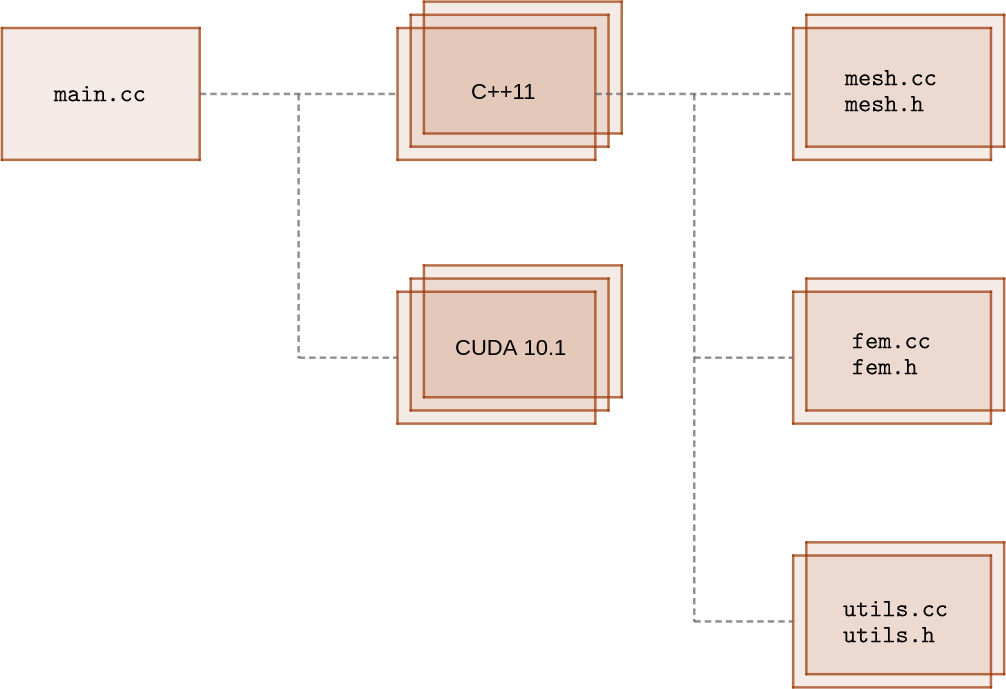
\includegraphics[width = 0.7\linewidth]{Figures/cpp_code}
	\caption{Code structure of the C++ code implementation.}
	\label{fig:cpp}
\end{figure}

Figure~\ref{fig:cpp} illustrates the overall design structure of the code - in both serial and parallel, though the GPU code will be discussed in more detail in Section~\ref{gpucode}. The code is split into four main files and their respective headers,
\begin{itemize}
	\item \texttt{main.cc} - Main C++ code, used for invoking the FEM operation and calling results to be output.
	\item \texttt{mesh.cc} - Contains the code for the Mesh class, storing all necessary operations and data structures to construct a mesh.
	\item \texttt{fem.cc} - Code for a FEM class which contains the routines needed to perform the method on a given mesh.
	\item \texttt{utils.cc} - General utility functions, such as SSE, parsing of command line arguments et cetera.
\end{itemize}
The approach here would be that a Mesh object be created, passed to a FEM object as an input parameter to a constructor, the FEM would complete the routine and the utility functions would perform sundry operations after this to tidy up. Figure~\ref{fig:serial_flow} demonstrates a flowchart of the serial code process.
\begin{figure}
	\centering
	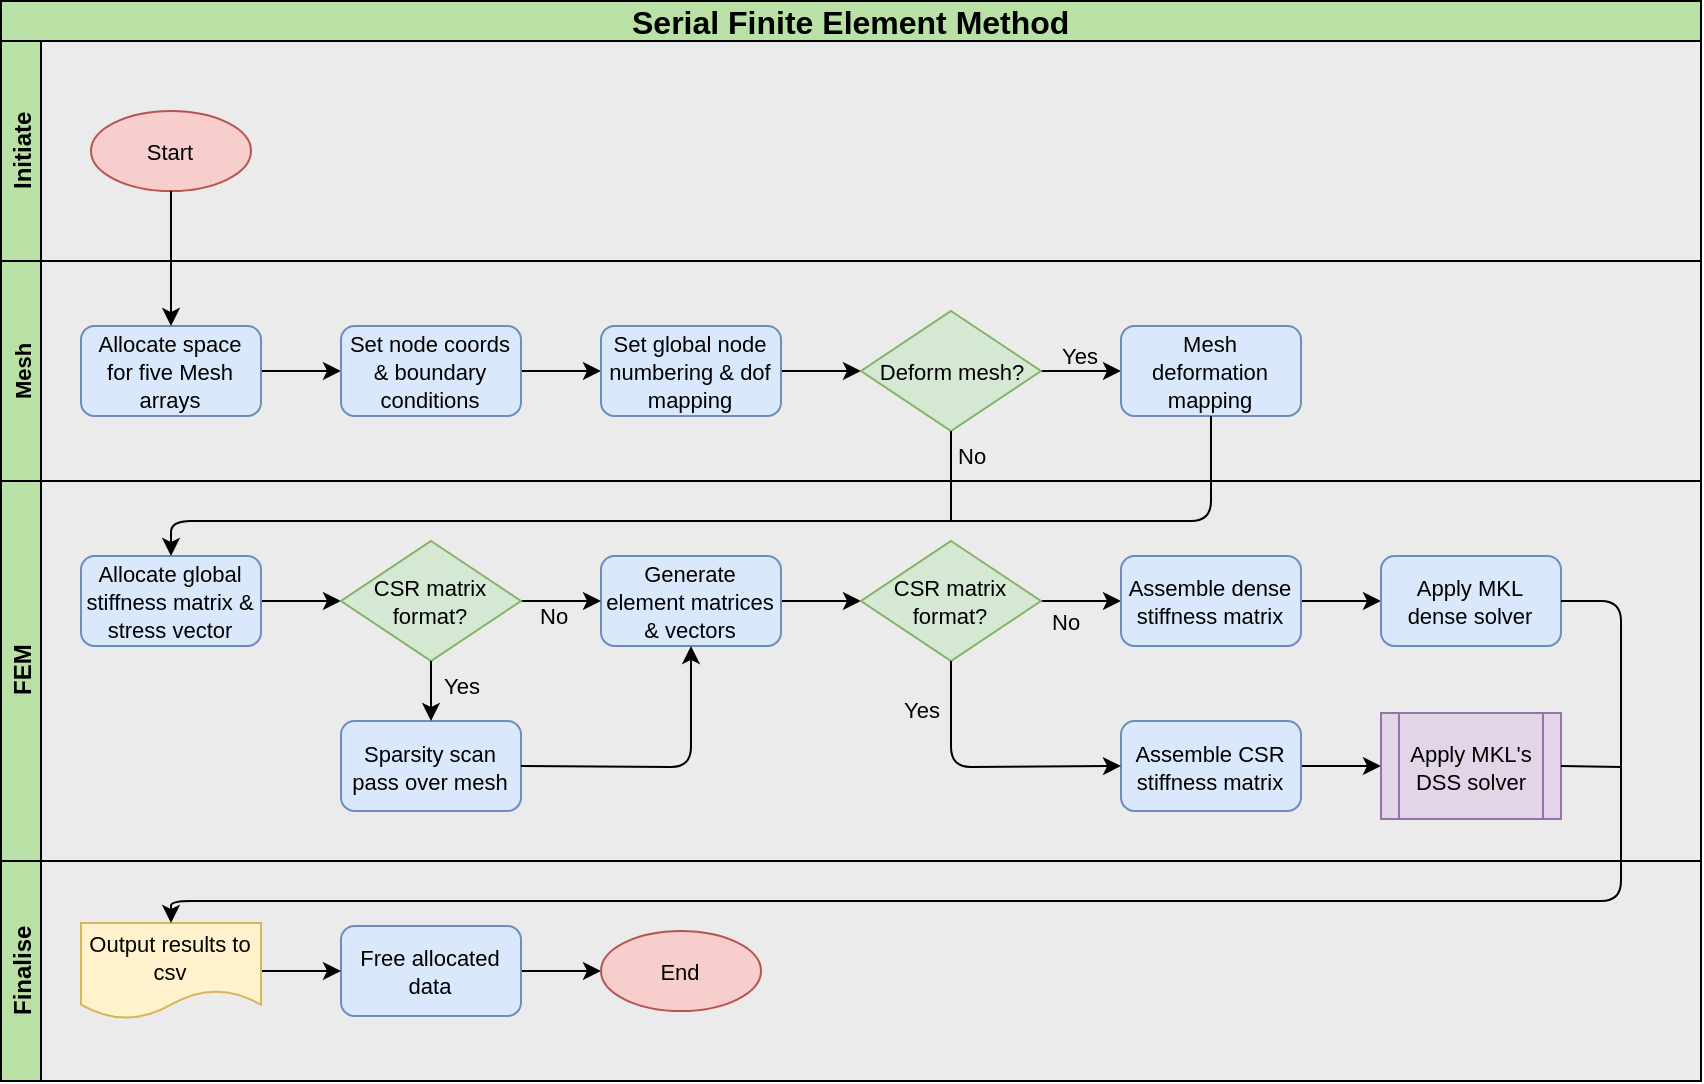
\includegraphics[width = 0.9\linewidth]{Figures/serial_flowchart}
	\caption{Flowchart of serial FEM implementation.}
	\label{fig:serial_flow}
\end{figure}

\section{Data Structures}

Objects are a massive sell for using C++ over C when programming a numerical method, for reasons stated already. For this paper, two classes were written, one to handle the mesh creation and one to handle performing FEM. In terms of other data structures, there was also a struct \texttt{Tau} to manage timings of all the operations without needing to pass around multiple variables in as function parameters.

\subsection{Mesh}\label{mesh}

The mathematics of the mesh has been illustrated, the next logical step would be to port it over to code. The data structure for the mesh holds a handful of key components and routines needed for its generation. Given the mesh itself is of course, a collection of interconnected nodes on a plane, upon each of which numerical calculations must be performed, it was naturally necessary to stores these nodes and their corresponding coordinates. In the implementation of this paper, a 2D mesh was used, though the extension to higher dimensions is rather arbitrary - another benefit of the FEM. The nodes' coordinates were stored in an array, \texttt{vertices}, which had a dimension of \texttt{order}, where order is the number of nodes or number of unknowns. Looking back at the Section~\ref{elems}, however, simply knowing the nodes coordinates for the FEM isn't enough, one also needs to know their global indices and degree of freedom mapping back to the stiffness matrix. These were respectively stored in two 2D arrays, \texttt{cells} and \texttt{dof}. Note that this is the exact same as performing the mapping function $q(e,r)$ seen previously. For example, \texttt{dof[e][r]} will provide the global node index of local node $r$ in cell $e$. Figure (REFERENCE) gives an example of a small mesh, the populated version of these three arrays are described in (LISTING). Note also in this example that each cell's array is numbered in an anti-clockwise direction - this is important for the orientation of the integrals calculated later. Since in this paper, only P1 examples were used, the degree of freedom mapping and global node indices are actually equal and so having two separate arrays for these was rather unnecessary but it allows for potential further expansion of the code with ease.

\begin{remark}
	Standard library vectors were not used for the 2D arrays as the contiguity of the data was important for transferring the data to the GPU and for certain linear solvers.
\end{remark}

In terms of what routines are contained in the Mesh class, during instantiation, the constructor creates a generic, rectangular mesh and populates the three arrays. There is a routine, whereby one can pass a mapping function as a parameter and deform the mesh. The aim of the deformation function is simply the fact that most FEM meshes aren't standard rectangles, apart from this particular test case - since the focus here is on a GPU optimisation. Other routines in the class then are merely to return various properties of the object: coordinates, pointers to the arrays (for CUDA purposes), number of nodes et cetera. There is also a routine to do a pass over the mesh and return its sparsity pattern which is detailed in Section~\ref{sparsity}.

\subsection{FEM}

Once the mesh has been generated, the next aim for the software was to create as generic a FEM class as possible, one which could take any mesh in the structure of the Mesh class, and solve the given PDE - in this report's case the Laplace equation. The FEM class will, of course, need to allocate data to store the global stiffness matrix and global stress vectors. The stress vector is simply stored in \texttt{b} and has a dimension of \texttt{order}, the stiffness matrix on the other hand can be stored in either dense or CSR format. Since CSR is stored in three separate, single dimensional arrays, this allowed the benefit of using standard library vectors, also eliminating the need for \texttt{new} and \texttt{delete}. The dense format on the other hand is 2D and has the same issue with contiguity as mentioned in the remark above. The CSR matrix is stored in \texttt{valsL}, \texttt{rowPtrL} and \texttt{colIndL} and the dense matrix is stored in \texttt{L}. The class then also stores certain properties needed, such as the dimensions of the problem \texttt{order}, the number of cells in the mesh and the number of non-zeros in the sparse matrix.

From a routine perspective, this is where all the real nuts and bolts of the FEM come into play.  There are three primary routines here which need to be completed in order to obtain a solution:
\begin{enumerate}
	\item element matrix generation.
	\item global stiffness matrix and stress vector assembly.
	\item linear system solver.
\end{enumerate}
The element matrix calculation is detailed in Algorithm (REFERENCE), utilising the convenient formulas stated in Section~\ref{problem}. The assembly routine on the other hand, has two different variants, one to handle the dense matrix assembly and one to handle assembling in CSR. Algorithms (REFRENCEx2) show both variants of this assembly. The last main routine, solving the linear system was handled by Intel's MKL library, taking advantage of pre-existing, optimised kernels.

\section{Sparse Storage}\label{sparse}

\begin{figure}
	\centering
	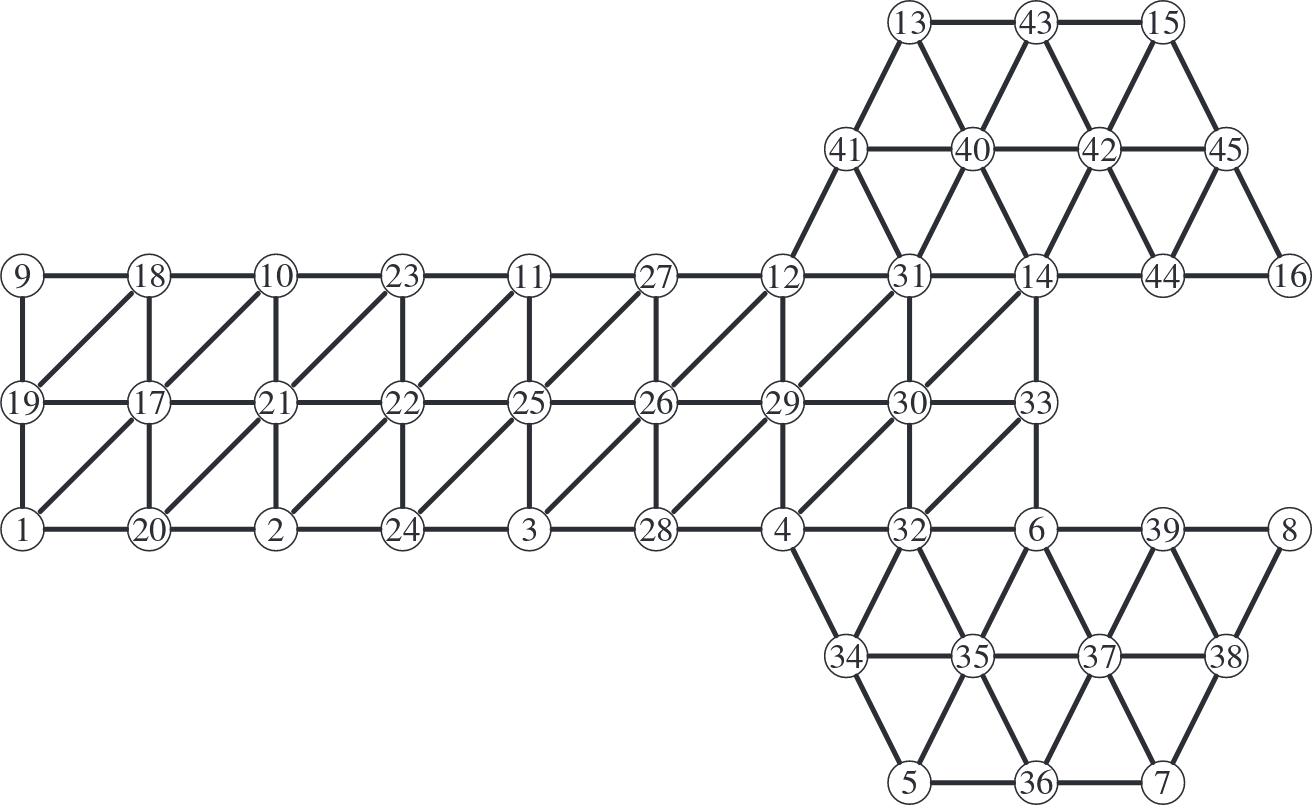
\includegraphics[width=0.7\linewidth]{Figures/mesh_graph}
	\caption{Mesh for generic FEM problem illustrated as a graph representation.}
	\label{fig:graph}
\end{figure}
\begin{figure}
	\centering
	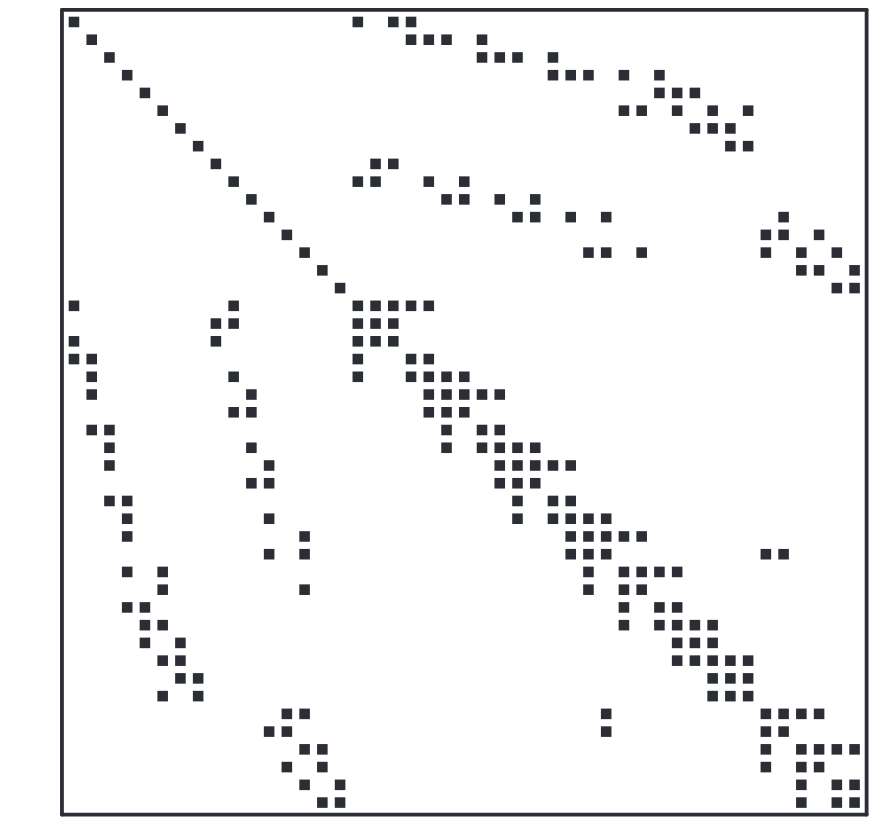
\includegraphics[width=0.4\linewidth]{Figures/sparsity_pattern}
	\caption{Sparsity pattern of FEM mesh.}
	\label{fig:pattern}
\end{figure}

The idea of sparse matrices and CSR storage has been thrown about in this paper a handful of times. The idea here is that a matrix is considered sparse, if if consists of mostly 0 valued entries - in some papers it is defined as having over 50\% 0 entries but this is a rather loose definition. This is important in the FEM as, if the basis functions are considered, one must remember that these are defined on a compact support $\Omega^{(e)}$, and will be 0 everywhere outside of this domain. Due to this, the global stiffness matrix will be a SPD, sparse matrix. Consider again Figure (REFERENCE), at no point is there any connection between nodes X and Y, thus the resulting inner product $\left\langle\varphi_X,\varphi_Y\right\rangle=0$. Why is this important? It can be hugely beneficial to computation time if one can take advantage of the sparsity pattern of a matrix, clearly as there is going to be potentially orders less null operations to iterate through.

These matrices can be stored in a number of different ways, three will be looked at here, although only CSR was used in the implementation:
\begin{itemize}
	\item CSR.
	\item CSC.
	\item COO.
\end{itemize}
CSR or \textit{compressed sparse row} storage is the most commonly used variant of sparse storage. As mentioned, it works by storing the matrix into three separate arrays, $A$, containing all the non-zero values, $IA$, the indices of the beginning of each row in the array $A$ and has a length of $n+1$ where $n$ is the number or rows, and finally $JA$, the indices of the column each value in $A$ is in. For more clarity, consider the matrix,
\begin{equation}
	A = 
	\left[\begin{matrix}
		3 & 1 & 0 & 0 & 0\\
		0 & 20 & 15 & 0 & 1\\
		0 & 0 & 0 & 4 & 1\\
		9 & 1 & 6 & 8 & 0\\
		0 & 0 & 0 & 7 & 0\\
		0 & 0 & 0 & 0 & 11
	\end{matrix}\right],
\end{equation}
in CSR format this can be written as,
\begin{lstlisting}
 A = [ 3 1 20 15 1 4 1 9 1 6 8 7 11 ]
IA = [ 0 2 5 7 11 12 13 ]
IJ = [ 0 1 1 2 4 3 4 0 1 2 3 3 4 ]
\end{lstlisting}
In the case of this implementation, \texttt{valsL} = A, \texttt{rowPtrL} = AI and \texttt{colIndL} = IJ. An important thing to note is that these can be either 0-based indexing or 1-based indexing. Since this report didn't utilise any FORTRAN code, 0-based indexing was used in all cases.

\textit{Compressed sparse column} is almost identical to CSR storage, except it is column-major format instead. The same example matrix in CSC would give,
\begin{lstlisting}
 A = [ 3 9 1 20 1 15 6 4 8 7 1 1 11 ]
IA = [ 0 3 0 1 3 1 3 2 3 4 1 2 5 ]
IJ = [ 0 2 5 7 10 13 ].
\end{lstlisting}
Clearly here, IJ has dimensions $m+1$, where $m$ is the number of columns.

The last commonly used sparse storage format is \textit{coordinate lists} or COO, which stores the values and their coordinates in both row and column. Keeping with the same example gives,
\begin{lstlisting}
 A = [ 3 1 20 15 1 4 1 9 1 6 8 7 11 ]
IA = [ 0 0 1 1 1 2 2 3 3 3 3 4 5 ]
IJ = [ 0 1 1 2 4 3 4 0 1 2 3 3 4 ].
\end{lstlisting}
This can of course be done in either row-major or column-major directions.

\subsection{Graph Theory}

Looking at the sparsity of a matrix, this can be equated to graph traversal problems in graph theory. If we consider a graph problem $G(V,E)$, defined as a set of vertices,
\begin{equation}
	V = \{v_0,v_1,\dots,v_n\},
\end{equation}
and a set of edges $E$, consisting of pairs of vertices $v_i,v_j$, such that,
\begin{equation}
	E \subseteq V\times V.
\end{equation}
From a sparse matrix perspective, this graph can be thought of as the connectivity between elements in the matrix, i.e. if $\{v_i,v_j\} \in E$, then it can be shown that for a sparse matrix $A$, $A_{i,j}$ is non-zero. Looking at Figure~\ref{fig:graph}, demonstrating a mesh for a FEM problem in the form of a graph. Clearly all the edges and connectivity are clear from the figure, but this also gives us the inherent sparsity patter in the resulting matrix. Figure~\ref{fig:pattern} demonstrates this resulting global stiffness matrix. Thinking back to how the FEM, particularly its elements were defined, this result makes sense. The basis functions were defined on a compact support of touching nodes, so clearly if $\{v_i,v_j\} \notin E$, then the resulting inner-product,
\begin{equation}
	\left\langle \varphi_i, \varphi_j \right\rangle = 0.
\end{equation}

\subsection{Sparsity Scan}\label{sparsity}

Naturally, the next question needing to be posed is, how does one take advantage of this inherent sparsity pattern available in the stiffness matrix. The easiest, although there have been papers published on more advanced methods (CITE), is to run a single pass over the mesh to begin, taking the computational hit, and using this to create a sparsity pattern. In this implementation, the pass created a vector of STL sets, one set for each node, and iterated through each, amending to the set if there was an edge between the two nodes. Using this, one now has the number of non-zeros and can populate quite easily, IA and IJ, in the CSR matrix. Algorithm (REFERENCE) details how this is explicitly performed.

\section{Solver Libraries}

A substantial part of the computation time in the FEM, relies on actually solving the final linear system. While this report is aimed at optimising the FEM in general, it does not aim at optimising linear solvers - something which has been covered by countless PhD students and doctors over many years. Instead, a decision was made to simply use a pre-existing library for both convenience and efficiency's sake. There are many variants that could have been used, GNU Standard Library, MAGMA, LAPACK etc. The one which was used in the end was Intel's MKL.

\subsection{Intel's MKL}\label{mkl}

The Intel library was split into two separate sub-libraries: their LAPACK routines for dense systems, and their Direct Sparse Solver (DSS). Both were used in this paper for comparison reasons. In either case, given that the stiffness matrix $A$, is symmetric positive definite (SPD), both dense and sparse solvers work by initially factorising the matrix using Cholesky decomposition, $A = L^T L$, where $L$ is lower-triangular. This new system is now solved using a direct solver. The DSS also has an option of providing a reordering of the sparse matrix, prior to the Cholesky decomposition, such as Cuthill-McKee (CITE), if one so wishes to make the sparsity pattern more compact, and thus more efficient for solving. Figure~\ref{fig:ordering} demonstrates the potential benefits of reordering, a much more compact data set, allowing for far more coalesced operations and less distance to travel along memory (CITE MATLAB SITE). This option was left on "auto" for the purposes of this report. 
CITE INTEL'S DOCUMENTATION
\begin{figure}
    \centering
    \begin{subfigure}{0.49\textwidth}
        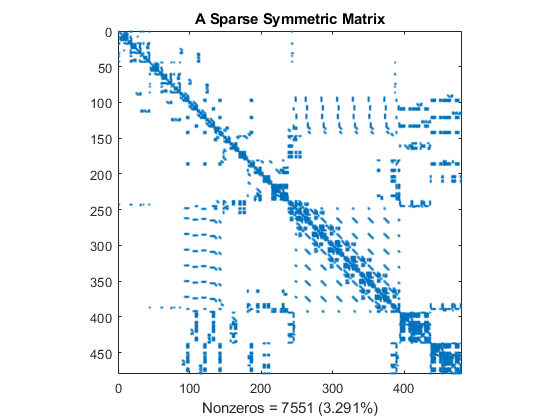
\includegraphics[width=\textwidth]{Figures/sparsity_unordered}
    \end{subfigure} \hfill
    \begin{subfigure}{0.49\textwidth}
        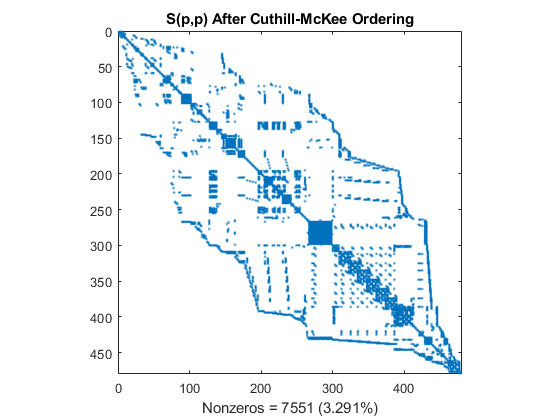
\includegraphics[width=\textwidth]{Figures/sparsity_cmckee}
    \end{subfigure} \\
    \begin{subfigure}{0.49\textwidth}
        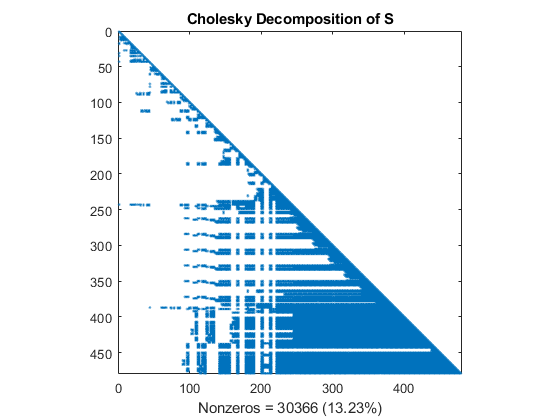
\includegraphics[width=\textwidth]{Figures/chol_unordered}
    \end{subfigure}\hfill
     \begin{subfigure}{0.49\textwidth}
        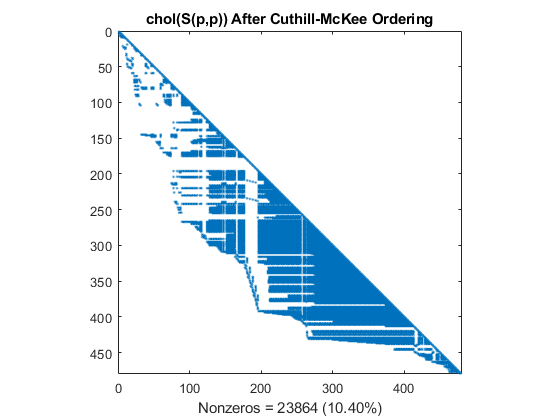
\includegraphics[width=\textwidth]{Figures/chol_cmckee}
    \end{subfigure}
    \caption{Illustration of a sparsity pattern of a matrix, pre and post Cuthill-McKee reordering, allong with the resulting Cholesky decompositions of both matrices.}
    \label{fig:ordering}
\end{figure}

\clearpage
\chapter{GPU Implementations}

In scientific computing, GPU programming can be hugely beneficial to large-scale problems. Due to the highly parallelisable architecture of GPUs, massive speed-ups can be seen. In this chapter, the heterogeneous, GPU programming model is discussed, as well as how this can be then implemented to apply the FEM. The design structure of the code written for this paper is detailed, as well as going through the theory of existing approaches.

\section{GPU Programming \& CUDA}

In GPU programming, there are multiple options currently available. Currently on UNIX systems, the main two would be CUDA and openCL, others exist such as openGL and DirectX. They each have their own benefits, openCL is open source and can be used on any device with graphical processing abilities, from a phone to a cluster, while CUDA is only available solely for Nvidia devices. While all having their differences, they do all share the same general approach, this section details the model needed to program a GPGPU over a CPU.

\subsection{GPU Programming Model}

\begin{figure}
	\centering
	\begin{subfigure}{0.35\linewidth}
		\centering
		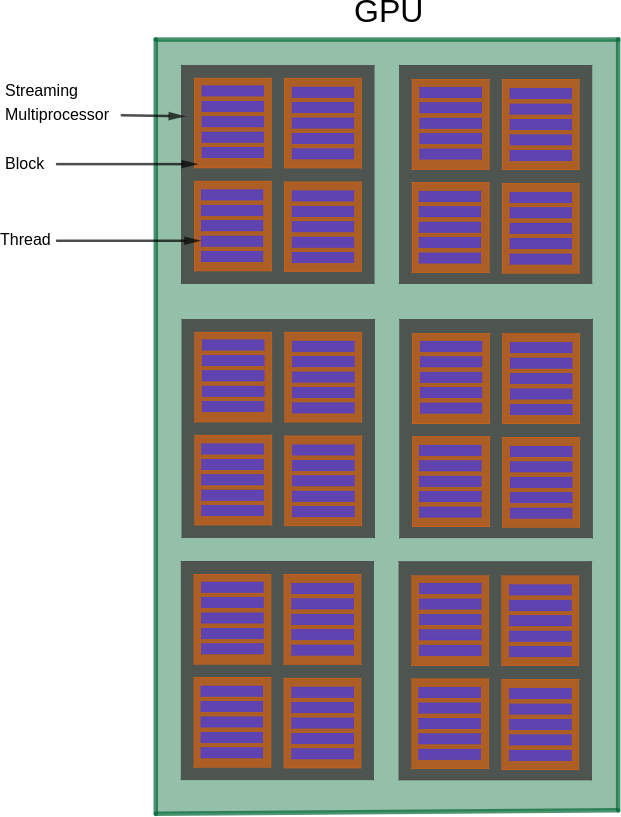
\includegraphics[width=\linewidth]{Figures/gpu_arch}
	\end{subfigure} \hfill
	\begin{subfigure}{0.55\linewidth}
		\centering
		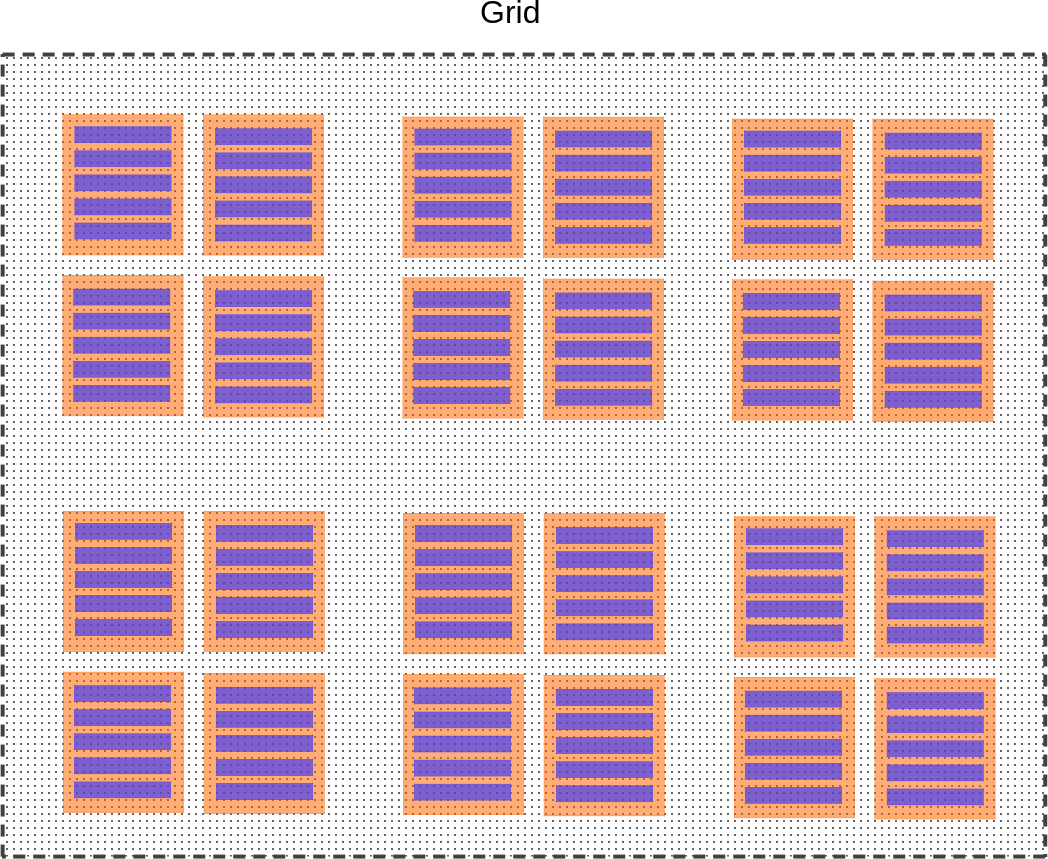
\includegraphics[width=0.9\linewidth]{Figures/gpu_grid}
	\end{subfigure}
	\caption{Illustration of a GPU's architecture and virtual grid. (NEED BETTER CAPTION}
	\label{fig:gpu_arch}
\end{figure}
While, as stated, GPUs have the potential to provide huge speed-ups, this is not necessarily a given. There is much to consider as a programmer when writing code which are not traditionally have to consider when writing code for CPUs - in serial, shared memory or even distributed architectures. CPUs traditionally consist of multiple cores, usually to the order of four to sixteen, sitting on a chip, with CISC architectures - meaning it is written to perform complicated instructions at with high clock speeds. These chips often contain up to three levels of automated caches, with buffers, preventing thrashing by first-in-first-out or least-recently-used strategies. They regularly have extra chips called accelerators for performing specific calculations like cryptography or data compression and can have quite complex scheduling algorithms. In short, CPU chips are very clever, but fall down when it comes to high levels of parallelism.

GPUs, on the other hand, are made up of thousands of CUDA cores, sitting on what are known as Streaming Multiprocessors - often about eight or so per SM. Each of these SMs are arranged into blocks of threads, making up an overall grid. The threads inside each block are what allow these massive amounts of parallelisation. On the current Turing architectures, a block can have a max of up to 1024 threads per block, for example. Considering that there can be thousands of CUDA cores, it is now  how this can be hugely beneficial. Figure~\ref{fig:gpu_arch} shows this architectural design structure. So what is the downside? The first, and most evident thing to consider, is these cores are very basic. They have SIMD instruction sets, similar to RISC on CPUs, multiple less complex control units and have slower clock rates. GPUs do also have accelerators on them, such as the newer Tensor Cores and Ray Tracing cores, as seen in Figure~\ref{fig:turing} showing Nvidia's diagram of the Turing architecture, but these are relatively recent and not much used as of yet. Figure~\ref{fig:cpugpu} shows a relatively basic illustration of the difference in architectures, illustrating the larger, more complex control unit, shared cache as well as the much larger \textit{arithmetic logic units} - threads in a GPU's case.

\begin{figure}
	\centering
	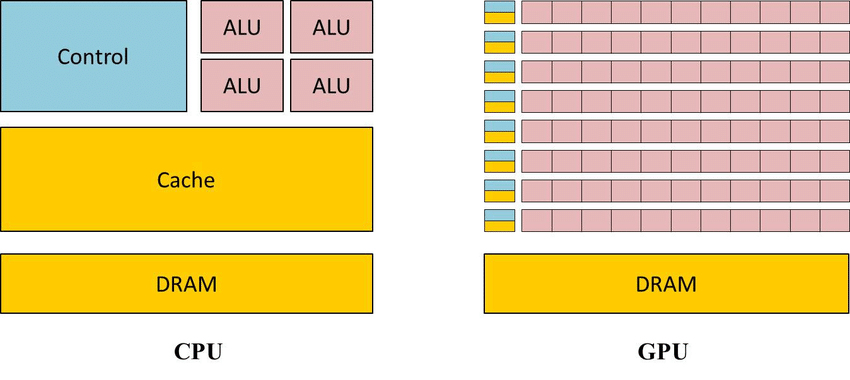
\includegraphics[width = 0.8\linewidth]{Figures/cpuvsgpu}
	\caption{Simplistic comparison of CPU vs. GPU architectures.}
	\label{fig:cpugpu}
\end{figure}
\begin{figure}
	\centering
	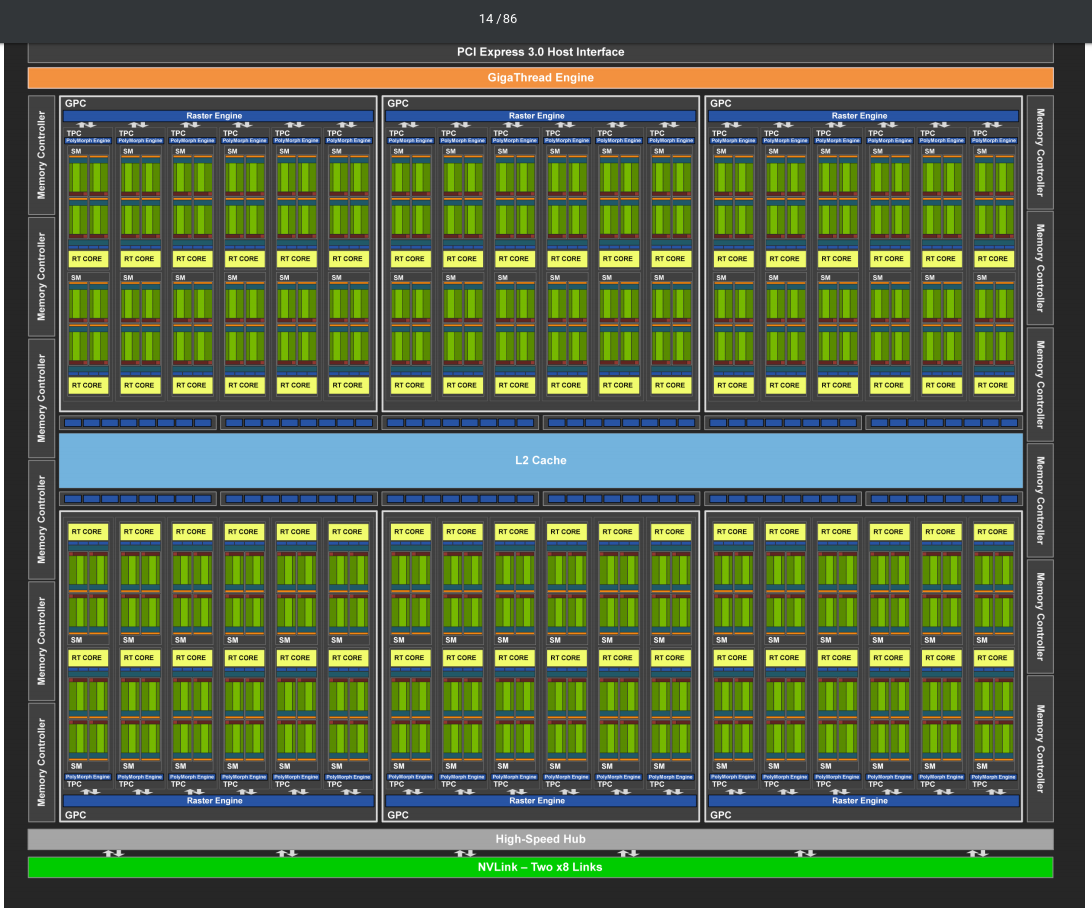
\includegraphics[width =0.65\linewidth]{Figures/turing}
	\caption{Illustration of Nvidia's current Turing architecture, showing its SMs and Ray Tracing cores.}
	\label{fig:turing}
\end{figure}

While slow clock-speed and simple instruction sets are the main drawbacks of using a GPU, there are other considerations to be made. The first, and almost certainly the most important when it comes to writing fast CUDA code is memory management. Unlike in Von Neumann, and other more modern CPU architectures, all of the memory management is left up to the programmer on a GPU and comes in various hierarchical levels. The largest bank of memory is \textit{global memory}, this is akin to the RAM of the GPU in terms of capacity order and is the slowest memory to access as it is physically furthest from the cores. The benefit of global memory is it is both the largest and also accessible to all cores on the card. There are other faster memory banks such as constant, texture, and surface which have various advantages and disadvantages such as being closer to the chip but non-programmable once set et cetera. However, there are two main types of memory which are most advantageous to take advantage of, \textit{shared memory} and \textit{thread registers}. Register memory is stored per thread and sits physically on top of the core. It is as fast as one can possibly get, but is limited in size. Similarly, shared memory also sits on top of the core, the main difference is that shared memory is distributed across all threads in a given block and is usually around 48KB in modern architectures. Figure~\ref{fig:mem} illustrates the memory hierarchy on a GPU. Unlike in CPUs, the programmer must decide where the various data needed to run the program will be stored, so clearly managing this correctly will be hugely important.

\begin{figure}
	\centering
	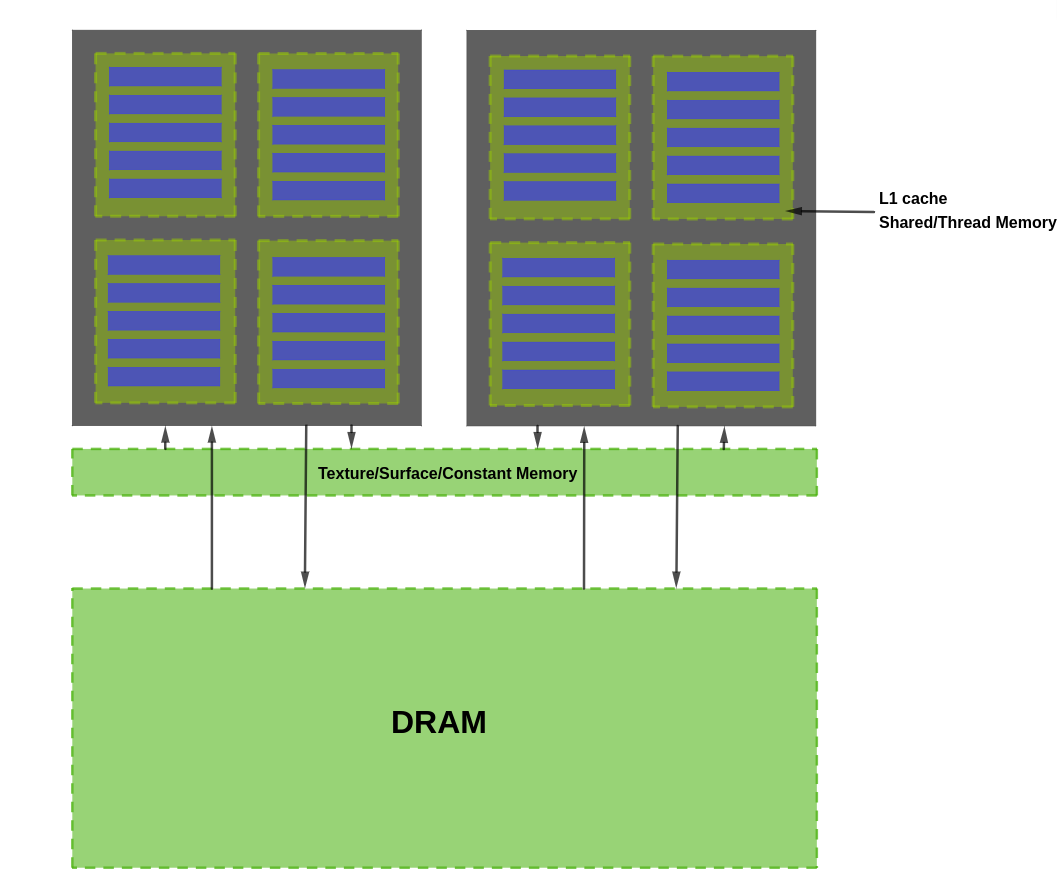
\includegraphics[width=0.8\linewidth]{Figures/mem_arch}
	\caption{CAPTION}
	\label{fig:mem}
\end{figure}

The final, main thing to consider, is what are known as warps. On the GPU, threads are organised into groups of 32. These groups of 32 threads all receive the same instructions at the same time. If some of the threads do not need to perform a given instruction, they will wait until the rest of the warp has completed the instruction until receiving another. Clearly, this can cause some bottlenecking. Figure (REFERENCE) demonstrates how this can apply to a specific case. The best thing one can do when taking warps into consideration is to attempt to set block sizes as multiples of 32 - since usually blocks are all performing the same or similar instructions.

In terms of actually putting this all to use, in CUDA, the code is structured by splitting the functions up into three classifications:
\begin{enumerate}
	\item \texttt{\twound host\twound} functions, are functions executed on the CPU or host. These are usually left without being denoted.
	\item \texttt{\twound global\twound} functions, also known as kernels. These are invoked by the host, and are a way of initiating the CUDA code - these are executed on the GPU. Usual inputs into these include, block and grid dimensions, shared memory allocation and streams.
	\item \texttt{\twound device\twound} functions are GPU functions which are called on by the device - these cannot be called by the host.
\end{enumerate}
Clearly then, the main difference between programming on a CPU compared to on a GPU is the onus put on the programmer to manage scheduling and memory management amongst other things without the assistance of the device. Thus, CUDA code must inevitably be more basic and more-so a collection of simple executions - it lends itself best to large scale operations of basic calculations.

\subsection{CUDA Libraries}\label{culibs}

While many of the GPU programming variants like openCL and openGL have their pros and cons, the main reason for choosing CUDA for this paper is, for one, Nvidia cards were used for testing so the performance would be optimal, but more-so due to the extensive availability of libraries for CUDA - something which openCL does not have. Intel's MKL was discussed in Section~~\ref{mkl}, and likewise, CUDA has its own collections libraries of mathematical functions. In Nvidia's case, these span from LAPACK, fast-Fourier transforms to image decomposition. In the case of this paper, cuBLAS, cuSOLVER and cuSPARSE were used. This is discussed in the breakdown of the GPU code's design structure in Section~\ref{culibs}. Similarly to the serial code, these were used for getting the Cholesky decomposition of a linear system and applying a direct solver. The cuBLAS package was used for finding the 2-norm of the error for each iteration seen in FEMSES.

\section{Current FEM Approaches}\label{approaches}

\subsection{Linear System Decomposition}

\subsection{Multigrid Techniques}

\subsection{Domain Decomposition}

\section{FEMSES}

The finite element method single-element solutions (or FEMSES) approach is the key study in this paper. Developed with the aim of decoupling solutions to the element matrices, from assembling the global stiffness matrix, aiming to reduce a large computational cost from the existing methods seen in Section~\ref{approaches}.

Traditionally, the FEM has four main steps: create the mesh, generate the element matrices and element vectors, assemble the global stiffness matrix and stress vector and lastly, solve the linear system. Of course, the global stiffness matrix and stress vector can be quite a large linear system, the idea of FEMSES is to decouple this from the overall process by implementing a 2-step iterative relaxation scheme on the element matrices, applying a Jacobi iteration to get estimates of the local solutions, and then assembling these using a weighting to achieve an estimate of the global solution. This step is repeated until convergence, thereby relieving the need to assemble the global stiffness matrix. Once convergence is achieved, the global solution is passed back to the host in one single transfer. The approach is identical to ones seen previously up until the point of actually assembling the global stiffness matrix.

\subsection{Two-Step Iterative Relaxation}

The two-step iterative relaxation scheme is, naturally, going to be the most dominant kernel seen in the approach. However, the premise is that it should be more efficient than needing to apply the Cholesky decompositions and a direct solver on the entire system. Consider the Jacobi iterative scheme,
\begin{equation}
	x^{\text{(new)}} = M^{-1}(b - N x^{\text{(old)}}),
\end{equation}
for the linear system $Ax=b$, where $M = \text{diag}(A),~N=A-M$ is a matrix splitting. For our linear system for the FEM, $Lu = b$, now define local element solutions as $u_e$. If now, the Jacobi method is modified slightly, we can write it as,
\begin{equation}\label{jacobi}
	u^{\text{(new)}}_e = M^{-1}(b - N u^{\text{(old)}}).
\end{equation}
It may seem strange here, to have an estimate to the global solution on the RHS and a the local solutions' estimate on the left. However, failing this, what will result is  if one takes, for example, the Laplace equation where the RHS of the linear system $b$, is mostly sparse, barring cells which have boundary conditions, a collection of trivial matrices. The solution will be given for all internal cells as the initial and so in order to take account for the entire mesh, the global solution must be used for the RHS.

\begin{figure}
	\centering
	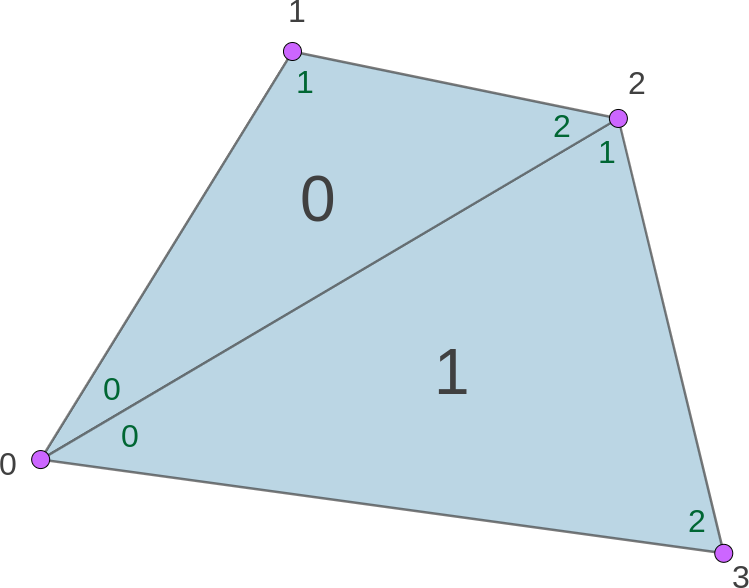
\includegraphics[width = 0.35\linewidth]{Figures/2cell2.png}
	\caption{Small two cell example of a mesh with global and local node numberings illustrated. NOT FINISHED}
	\label{fig:2cell2}
\end{figure}
The second step in the 2-step iterative relaxation is to take these local solutions, and assemble them into a global solution. This is done by creating a weighting array, summing up the contribution of each node on the denominator. Mathematically, the weighting and assembly is given by,
\begin{equation}\label{weight}
	u_i^{(new)} = \sum_e^{q(e,r) = i}\frac{A^{(e)}_{r,r}}{w_i} (u_r)_e^{(old)},
\end{equation}
where,
\begin{equation}
	w_i = \sum_e^{q(e,r) = i}A^{(e)}_{r,r}
\end{equation}
Figure~\ref{fig:2cell2} illustrates a small two-cell implementation. In this example, the Jacobi relaxation for cell 0 is given by,
\begin{equation}
	\left[\begin{matrix}
		(u_0)_e^{(new)} \\
		(u_1)_e^{(new)} \\
		(u_2)_e^{(new)}
	\end{matrix}\right] = 
	\left[\begin{matrix}
		\frac{1}{A^{(0)}_{0,0}} & 0 & 0 \\
		0 & \frac{1}{A^{(0)}_{1,1}} & 0 \\
		0 & 0 & \frac{1}{A^{(0)}_{2,2}}
	\end{matrix} \right]
	\times (-\mathbb{I}_3)
	\left[\begin{matrix}
		0 & A^{(0)}_{0,1} & A^{(0)}_{0,2} \\
		A^{(0)}_{1,0} & 0 & A^{(0)}_{1,2} \\
		A^{(0)}_{2,1} & A^{(0)}_{2,1} & 0 
	\end{matrix}\right]
	\left[\begin{matrix}
		u_0^{(old)} \\
		u_1^{(old)} \\
		u_3^{(old)}
	\end{matrix}\right]
\end{equation}
and the assembly using the weighting for global node 2,
\begin{equation}
	u_2 = \frac{A^{(0)}_{2,2}}{A^{(0)}_{2,2} + A^{(1)}_{1,1} } (u_2)_0 + \frac{A^{(1)}_{1,1}}{A^{(0)}_{2,2} + A^{(1)}_{1,1} } (u_1)_1.
\end{equation}

\subsection{Advantages \& Limitations}

The advantages of this approach is it improves on the parallelism seen in other methods. Of course, like the other approaches, the element matrices may be built in parallel and stored in global memory. However, after this, the assembly and solution of the linear system requires quite a substantial amount of communication between threads and synchronisation whereas the local solution estimates may be calculated entirely in parallel. The assembly of the global solution from the weightings can also be done substantially in parallel barring some scattered atomic functions when adding back to the global solution array. These atomic functions should not cause much overhead either as they are not in sequential order, they are ordered depending on the shape of the mesh. This is detailed in Section~\ref{femses}.

On the other hand, in terms of drawbacks, the Jacobi iteration isn't the most efficient iterative method. It bodes well here due to needing to use two different vectors on the LHS and RHS, which might cause some complications in something like the Gauss-Seidel, as you don't have the most recent update until the global solution is assembled. However, it is rather slow to converge. There is also somewhat of a communication hit in the process. After each iteration is completed, convergence must be checked, since kernels cannot call recursively, the convergence check must pass back the error term to the host, in order to test if the loop shall continue or not. It isn't hugely costly as it is only a single float, but it is still a consistent amount of device-host synchronisations.

\section{Implementations}\label{gpucode}

As mentioned, there is a lot of machinery and parts to move around in applying the FEM, especially when applying it on a GPU. Due to this, all of the code was written in CUDA~10.1, to avoid unnecessary complications with openCL and to take advantage of the Nvidia CUDA libraries. Unfortunately, CUDA cannot handle C++ code like the serial approach can, but rather only in C, thus the operations had to be made as simple as possible, no STL features were used in the CUDA code. 

\subsection{Design Structure}

Figure~\ref{fig:cuda} illustrates the overall design structure of the CUDA code. The code was largely divided up into three main files and headers:
\begin{enumerate}
	\item \texttt{gpu\_fem.cu} - Contains the \texttt{\twound host\twound} functions and all the \texttt{\twound global\twound} and \texttt{\twound device\twound} functions for the general, FEM GPU approach - applying a linear decomposition to the linear system.
	\item \texttt{gpu\_femses.cu} - Contains the \texttt{\twound host\twound} functions and all the \texttt{\twound global\twound} and \texttt{\twound device\twound} functions for the FEMSES GPU approach.
	\item \texttt{gpu\_utils.cu} - Contains general utility functions for use in the two main methods, such as LAPACK and BLAS operations.
\end{enumerate}
Both \texttt{\twound host\twound} functions are \texttt{extern} functions and so either can be invoked from the C++ code in \texttt{main.cc}. Note also that there is code reuse of \texttt{\twound device\twound} functions, so the flag \texttt{--relocatable-device-code=true} had to be set during compilation. Other flags for the CUDA libraries also had to be enabled, similar to the MKL library flags seen in the serial code.
\begin{figure}
	\centering
	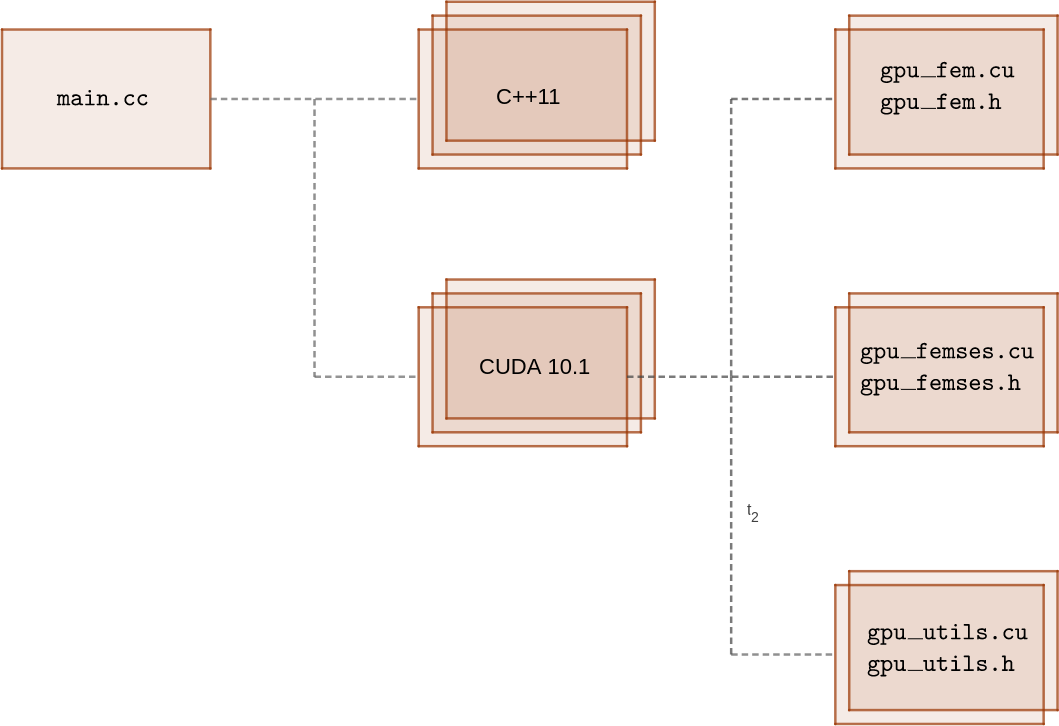
\includegraphics[width = 0.7\linewidth]{Figures/cuda_code}
	\caption{Structure of CUDA GPU code.}
	\label{fig:cuda}
\end{figure}

\subsection{Considerations}

There is a lot of data structures needed, so managing data reuse and reduction of transfers was a big consideration when designing the CUDA code. If something need not be transferred from host to device, it would be avoided. As well as this, the aim was to optimise shared memory use and minimise excessive synchronisation. For non-shared memory, attempting to keep the data coalesced is an important consideration as global memory access is quite slow. Fancy STL functionality couldn't be used so workarounds there had to be used - for example in the case of the sparsity pass function, this could not be performed on the GPU so it had to be done in serial and the resulting vectors transferred over. The last thing was to try minimise thread divergence from warps - reducing the amount of if statements is usually a good place to start along with making block sizes multiples of 32.

\subsection{Basic FEM}\label{basicfem}

\begin{figure}
	\centering
	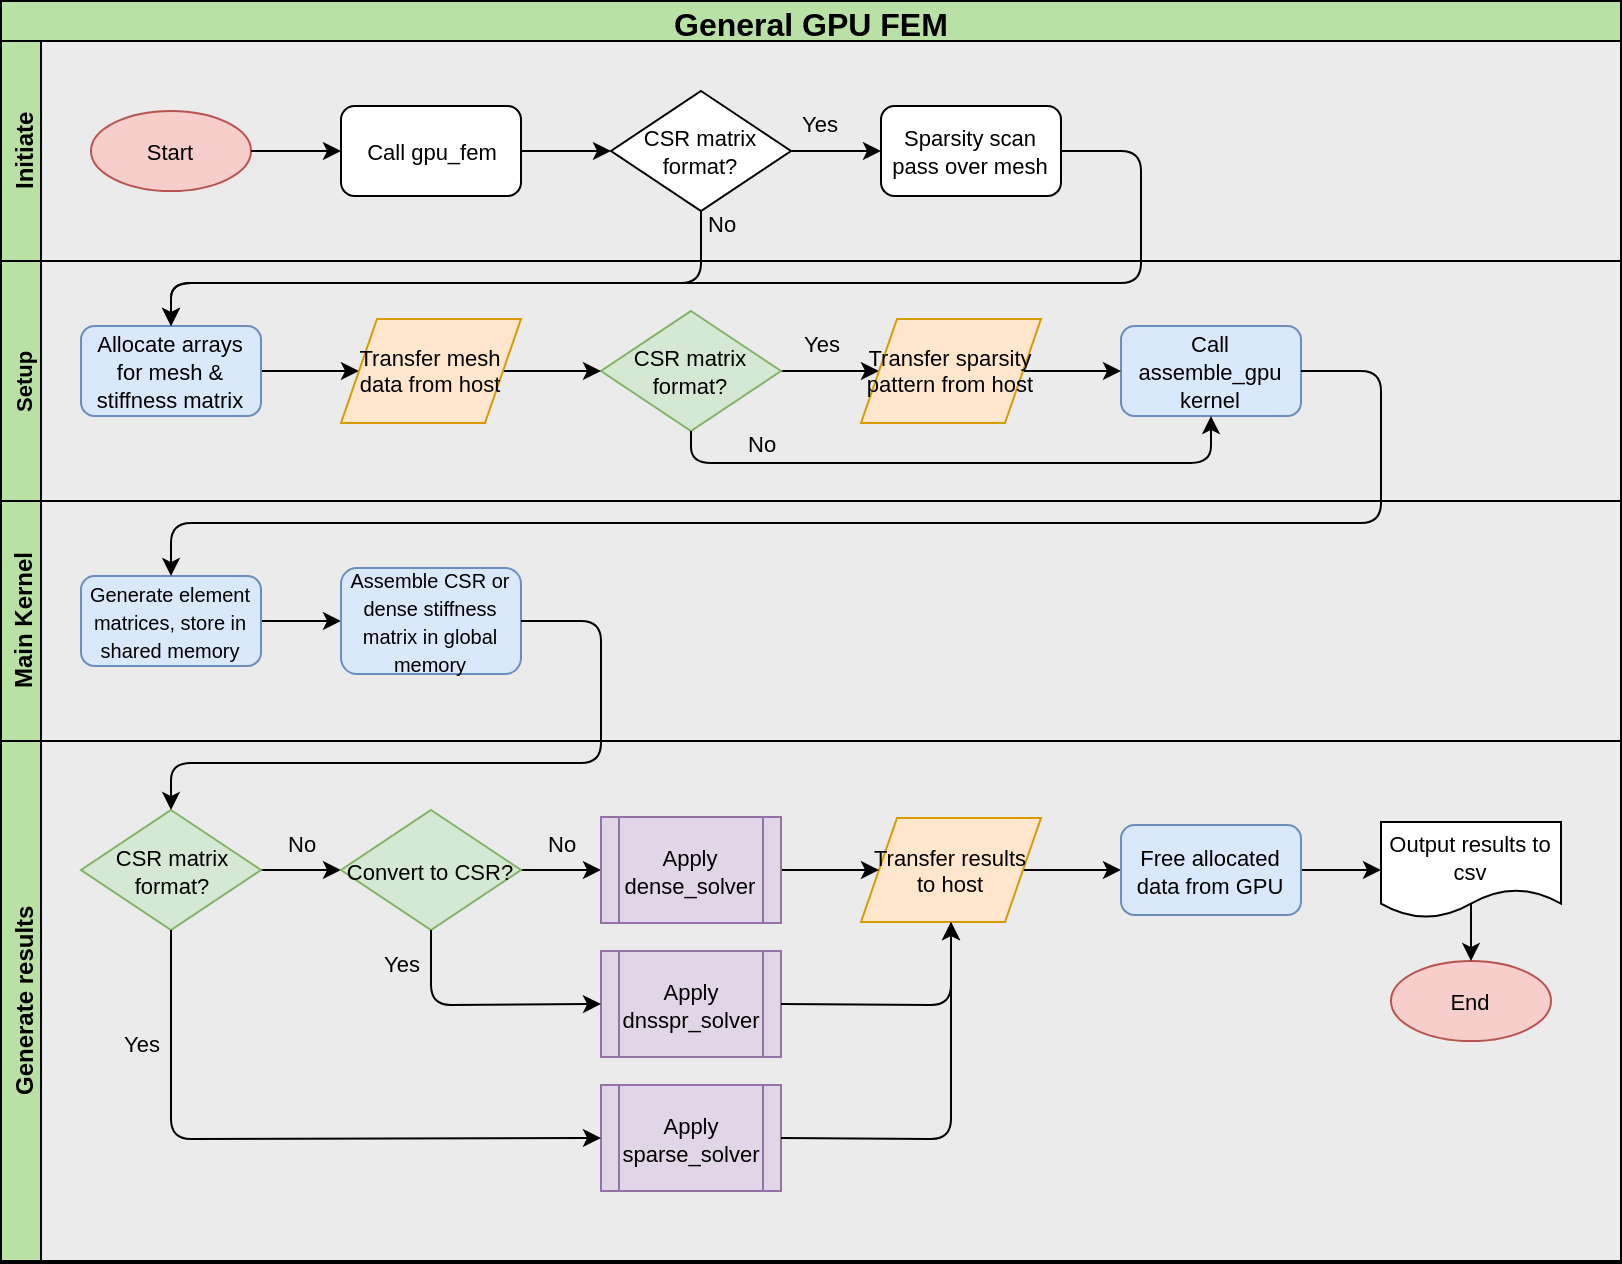
\includegraphics[width = 0.9\linewidth]{Figures/gpu_flowchart}
	\caption{Flowchart of general GPU FEM implementation.}
	\label{fig:gpu_flow}
\end{figure}
In Figure~\ref{fig:gpu_flow}, a flow chart of the approach taken to code a basic FEM implementation on a GPU is illustrated. The coloured steps the ones which are executed involving CUDA code, the white steps are ones which are executed entirely on the host. The generation of the mesh and all its pertaining information needed, is all completed in serial, which is then passed down to the device, and for the most part, barring a sparsity scan, the rest of the entire FEM process is completed on the device. The element matrices creation and stiffness matrix assembly is all completed in a single kernel. The linear system solution is then solved using cuSOLVER - and cuSPARSE depending on the matrix structure flagged at run-time. Once this is complete, the final solution is passed back to the host and the CUDA code is complete.

\subsubsection{Storage \& Memory Management - Mention solver taking up space}

\begin{figure}
	\centering
	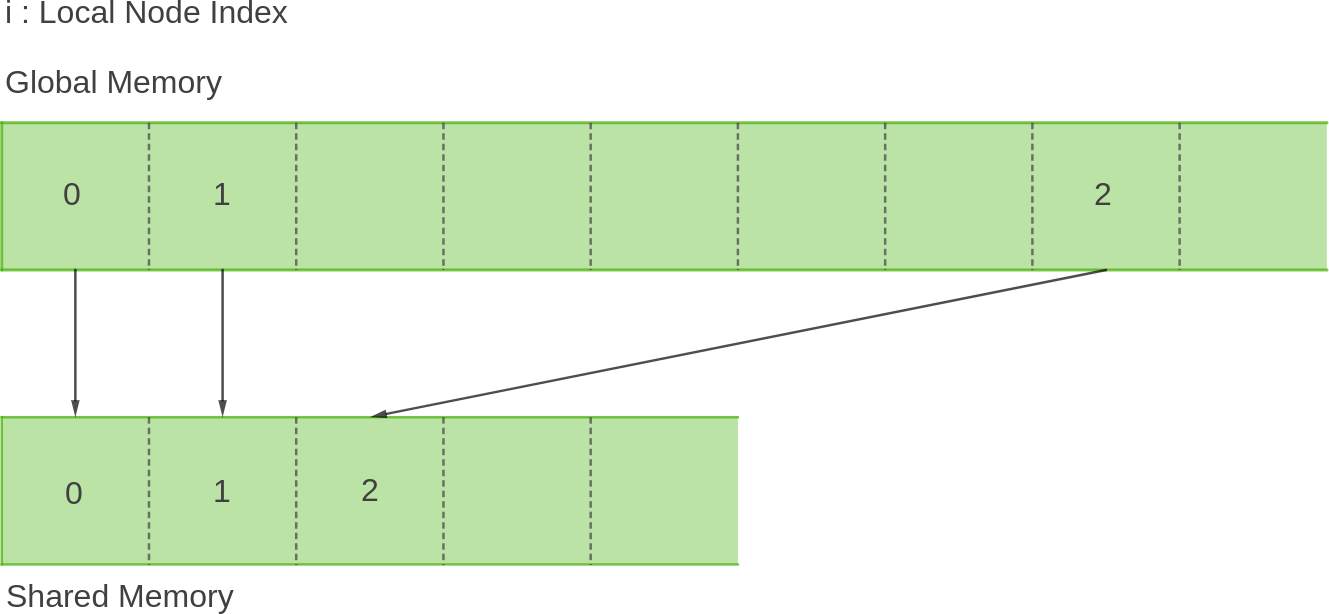
\includegraphics[width = 0.8\linewidth]{Figures/non_coalesced}
	\caption{CAPTION}
	\label{fig:coalesc}
\end{figure}
In terms of storage, for a problem which scales like FEM does, managing your resources correctly and not doing excessive memory allocations is important - along with, of course, freeing any allocations which are completed. The first thing needed to be allocated on the GPU is the five arrays to store the mesh. Exactly like was mentioned in Section~\ref{mesh}, memory needs to be allocated to store \texttt{vetices\_gpu}, \texttt{cells\_gpu}, \texttt{dof\_gpu}, \texttt{is\_bound\_gpu} and \texttt{bdry\_vals\_gpu}. In terms of memory being coalesced, all five arrays are indeed contiguous, and in both \texttt{cells\_gpu} and \texttt{dof\_gpu}, the memory access pattern is sequential so this won't pose any coalescence problems. However, the other three arrays, the memory access pattern jumps up and down the array, completely dependent on the shape of the mesh, and the connectivity of the nodes. Thus to handle this, as detailed in the device functions, the necessary values are read into shared memory in single writes to hedge this bottleneck. Figure~\ref{fig:coalesc} illustrates this, showing the lack of coalescence and the solution by writing to shared memory once.

Naturally, the next thing which needs to be allocated is the actual stiffness matrix itself. For this, unlike in serial, only the global stiffness matrix and stress vector need be allocated on global memory, since the local element matrices will be stored on shared memory. Depending on the choice to assemble a sparse or dense matrix will decide what must be allocated. For a dense case, a single dimensional array \texttt{L}, will be allocated, for the sparse case, three arrays must be allocated, \texttt{valsL}, \texttt{colIndL} and \texttt{rowPtrL}, as seen in Section~\ref{sparse}. The CSR matrix, unfortunately does not have coalesced memory access, but it makes up for this by the huge reduction in the actual size of the matrix, and so, the timing should scale far better than dense. Both dense and sparse allocated the same space for the stress vector, as it is stored in dense format. This will be overwritten with the resulting solution, saving the space for needing an extra array.

There is quite a large amount of data needed to be transferred from the offset in the FEM from device. All five of the mesh's arrays must be transferred from host to device (\texttt{dof\_gpu} technically does not when using P1 cases, but as stated this is to leave scope for further expansion). On top of this, as mentioned, the GPU cannot perform the sparsity scan algorithm, thus this must be done on the host. This algorithm populates both the column-index array and row-pointer array in the CSR structure, both of these must be transferred at the beginning when a sparse solution is chosen.

In terms of transfers, in both sparse and dense cases, the five arrays for the mesh need to be transferred. If \texttt{order} and \texttt{num\_cells} represent the number of unknowns/nodes and the number of cells respectively, then these five arrays take up,
\begin{flalign}\label{mem}
	\texttt{mem} &= \texttt{(3}\times\texttt{order}\times\texttt{sizeof(float))+(((6}\times\texttt{num\_cells)+order)}\times\texttt{sizeof(int))},&&\\
	\texttt{mem} &= \texttt{(14}\times\texttt{order) + (12}\times\texttt{num\_cells)},&&
\end{flalign}
where \texttt{mem} is measured in bytes. The two approaches  will then differ when it comes to storing the stiffness matrix and transfers. For both cases, the global solution array will need to be stored and also transferred back to the host, which will take up $\texttt{order}\times\texttt{sizeof(float)}$, or $\texttt{4}\times\texttt{order}$, bytes. This is the same array used to store the stress vector - it will simply be overwritten by the solution. For transfers, the sparse matrix must receive two arrays from the host after the sparsity pattern has been completed, the column-index array and row-pointer array, these are sized $\texttt{nnz}\times\texttt{sizeof(int)}$ and $\texttt{(order+1)}\times\texttt{sizeof(int)}$ respectively, where \texttt{nnz} is the number of non-zero entries achieved from the sparsity scan. The sparse approach also must store the values in \texttt{valsL}, taking up $\texttt{nnz}\times\texttt{sizeof(float)}$ too. There are no extra transfers needed for the dense approach but the memory needed to store the stiffness matrix is far larger, coming in at $\texttt{order}\times\texttt{order}\times\texttt{sizeof(float)}$. Therefore it can be said that the total amount of data needed to be transferred,
\begin{flalign}
	&\texttt{mem\_transf\_sparse} = \texttt{(20}\times\texttt{order) + (12}\times\texttt{num\_cells) + (2}\times\texttt{nnz) + 2},&& \\
	&\texttt{mem\_transf\_dense} = \texttt{(18}\times\texttt{order) + (12}\times\texttt{num\_cells)}, &&
\end{flalign}
and the total amount of memory allocated on global memory,
\begin{flalign}
	&\texttt{mem\_alloc\_sparse} = \texttt{(20}\times\texttt{order) + (12}\times\texttt{num\_cells) + (2}\times\texttt{nnz) + 2},&&\\
	&\texttt{mem\_alloc\_dense} = \texttt{(18}\times\texttt{order) + (12}\times\texttt{num\_cells) + (4}\times\texttt{order}\times\texttt{order)}.&&
\end{flalign}
This is an important factor to take into account when deciding what problem size to calculate as memory on the GPU is limited. In the case of the two GPUs tested in this report, the Tesla K40 has 12GB of global memory, while the GeForce RTX2080 Super has 8GB.

\subsubsection{Kernels}

There are two main kernels for this approach: the first kernel, \texttt{assemble\_gpu} or in its sparse form, \texttt{assemble\_gpu\_csr}, will take the input mesh as transferred prior, create the element matrices and assemble the global linear system, storing it back into global memory, this is demonstrated in Listing (REFERENCE); the second kernel, utilises CUDA libraries to solve the linear system. The assembly kernel was written specifically for this implementation, thus the setup of the grid and block dimensions must be set by the user. In order to take as much advantage of shared memory as possible, it was noted that the only real communication at this stage in the FEM process, is between nodes in the same cell. The setup of the kernel is then set that there are \texttt{block\_size\_X}, cells per block, in the $x$ direction, and 3 nodes per cell, in the $y$ direction. This gave the convenient benefit of \texttt{idx} being equal to the cell number, and \texttt{idy} being the local node numbering. This mapping is illustrated in Figure (REFERENCE). The kernel itself, runs two primary device functions, the first one generates the element matrices on shared memory, and the second then assembles these from shared memory into the global stiffness matrix, writing back to global memory. For two reasons, this is where the kernel had to terminate: you cannot globally synchronise the entire CUDA device within a kernel, only individual blocks, moving on to solve the linear system from here would almost certainly cause race conditions. The second reason is simply to avoid having to rewrite linear solver libraries that have already been optimised.

The linear solver kernel, comes in three different variations: one for CSR, one for dense matrices, and one which converts a dense matrix into CSR and solves. Unlike the assembly kernel, however, there is no need to decide how to organise the blocks and threads as this is taken care of by the library itself inside a variable called the handle, which is invoked at the beginning and passed into all library functions. In terms of what actual library functions are used, for the sparse solver, cuSPARSE is used to define the matrix structure, such as number of non-zeros, zero-based indexing, symmetric positive definite et cetera. This is used in tandem with cuSOLVER's single-precision, sparse SPD, Cholesky decomposition direct solver, \texttt{cusolverSpScsrlsvchol}. Unlike in the serial version, and Intel's DSS, the cuSOLVER kernel needs to store the entire matrix, as opposed to only the upper or lower half. This is an unnecessary bottleneck but one which cannot be avoided. The dense-CSR solver kernel, applies the same functionality as the sparse kernel, except for executing two other library kernels prior to the solver, \texttt{cusparseSnnz}, to deduce the sparsity pattern of the matrix, and \texttt{cusparseSdense2csr}, to convert from dense to CSR. The dense solver on the other hand, naturally does not use cuSPARSE. It does, however, split its solver kernel into two separate operations, the first being the actual Cholesky factorisation using \texttt{cusolverDnSpotrf} and the second applies the solver, \texttt{cusolverDnpotrs}. Figure~\ref{fig:cusolvers} shows flowcharts of the necessary steps required in order to execute the three solver variants.
\begin{figure}
	\centering
	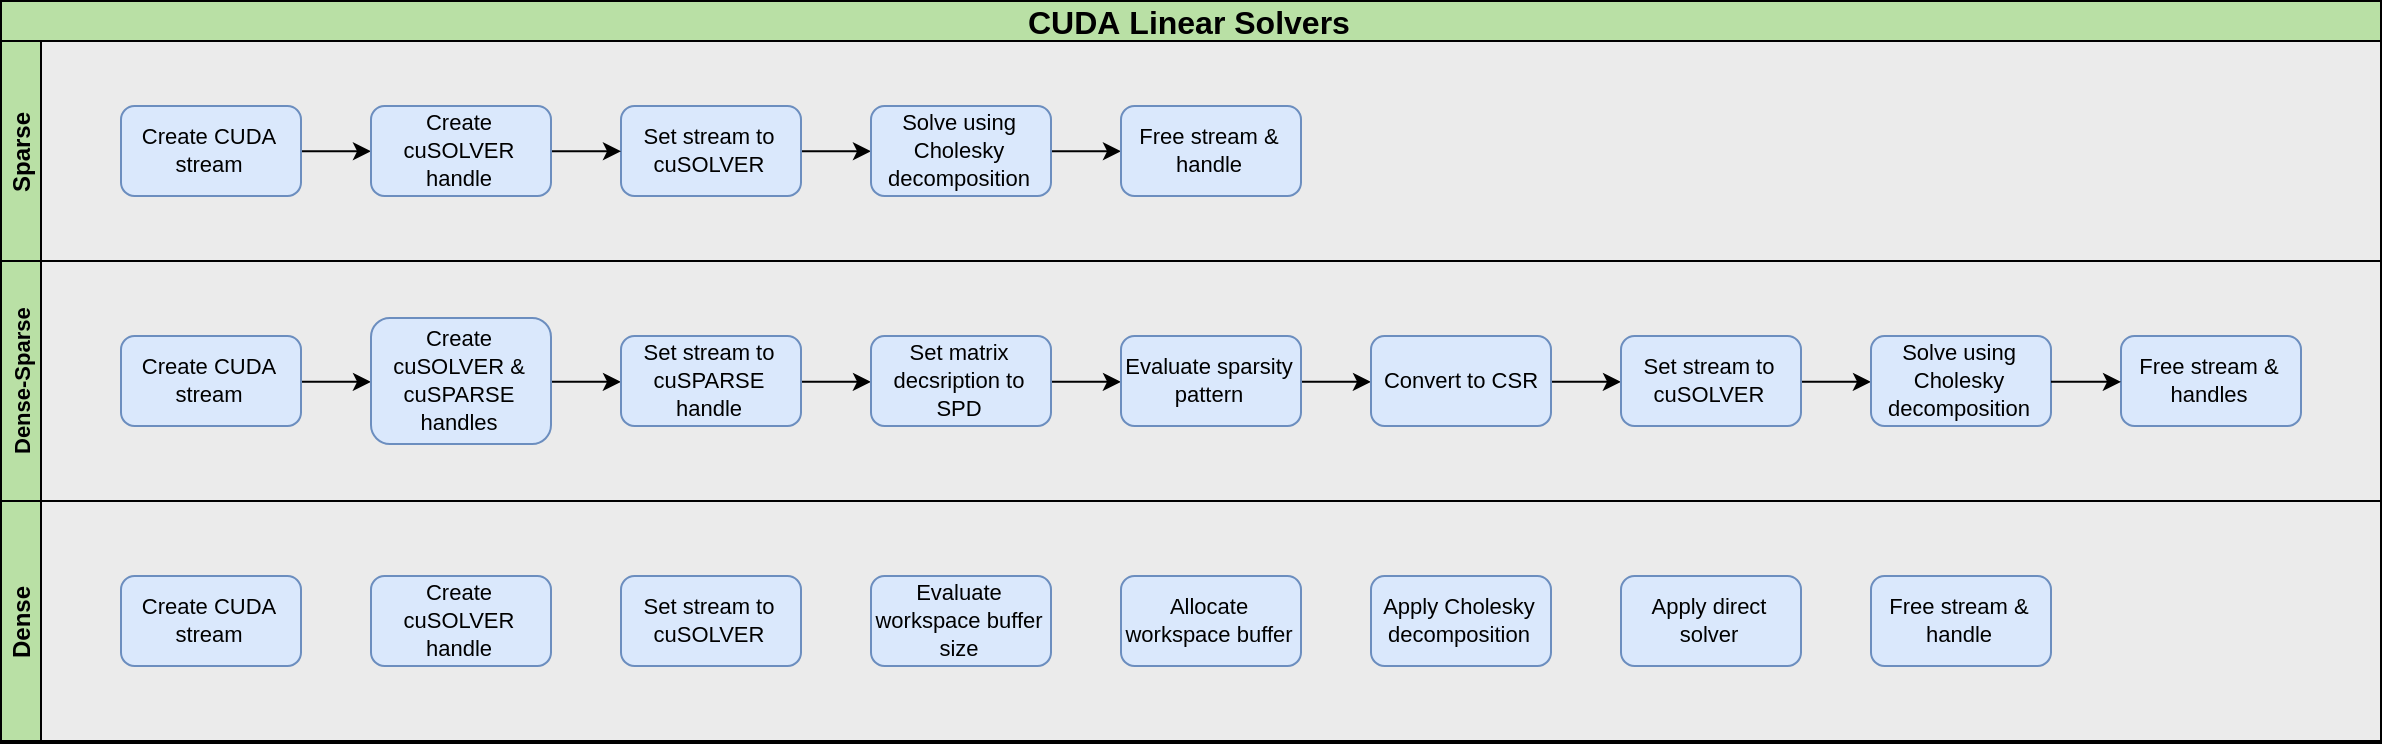
\includegraphics[width=0.9\linewidth]{Figures/cuda_solvers}
	\caption{Flowchart illustrating the steps needed to implement solvers from CUDA's linear algebra libraries.}
	\label{fig:cusolvers}
\end{figure}

\subsubsection{Device Functions}

There are two main device functions written for the assembly kernel. Prior to running these, when invoking the kernel the required amount of shared memory must be allocated. The grid structure is defined as \texttt{block\_size\_X} FEM cells per block, within each block there is one FEM cell designated per row of threads in the $x$-axis, and 3 nodes per row i.e. one node per thread in the $y$-axis. The shared memory needs to be large enough to store the element matrix \texttt{Le}, the element vector \texttt{be} as well as some other constants which need reuse such as the coordinates of each node in the cell \texttt{xi}, the global node numberings \texttt{dof\_r} and the constants seen in Equation~\eqref{conv}, for each cell in the block. Thus the amount of shared memory required is $\texttt{28}\times\texttt{block\_size\_X}$. This memory structure is displayed in Figure (REFERENCE) for an example block size of 4 in the $x$-axis. This would need to be larger of course, for non-P1 type problems but for this implementation it is sufficient.

The first device function, \texttt{assemble\_elem}, starts off by setting pointer values for the element matrices, element vectors and constants in shared memory. It reads in the global node numbering associated with the node for that particular thread into the thread register. It then reads in the coordinates of the three nodes in that cell into shared memory so that data is now coalesced and then synchronises the threads in the block. The area of the cell is calculated by the thread associated with local node 0, and then the $\beta$ and $\gamma$ values are calculated in parallel. After this point, the device function runs Algorithm (REFERENCE), where each thread calculates a single row in the element matrix and writes them to the shared memory array. Notice that there is need for atomic functions when enforcing the boundary conditions, this is to prevent race conditions as the threads need to write to the same memory addresses. 

A large speed-up point here is that the element matrices never need to be written to global memory, but rather the second kernel which assembles the global stiffness matrix simply assigns the pointers to the same location as the previous device function. For the assembly function, the global node numbers for the node associated with each thread are read in from global memory once and written over the constants in the previous function. Algorithm (REFERENCE) or Algorithm (REFERENCE), is then applied in parallel, depending on whether the matrix is dense or CSR, and written back to global memory. Again, unlike in the serial case, for the CSR matrix the entire matrix must be assembled and not simply its upper or lower-echelon form due to limitations of cuSOLVER.

\subsection{FEMSES}\label{femses}

\begin{figure}
	\centering
	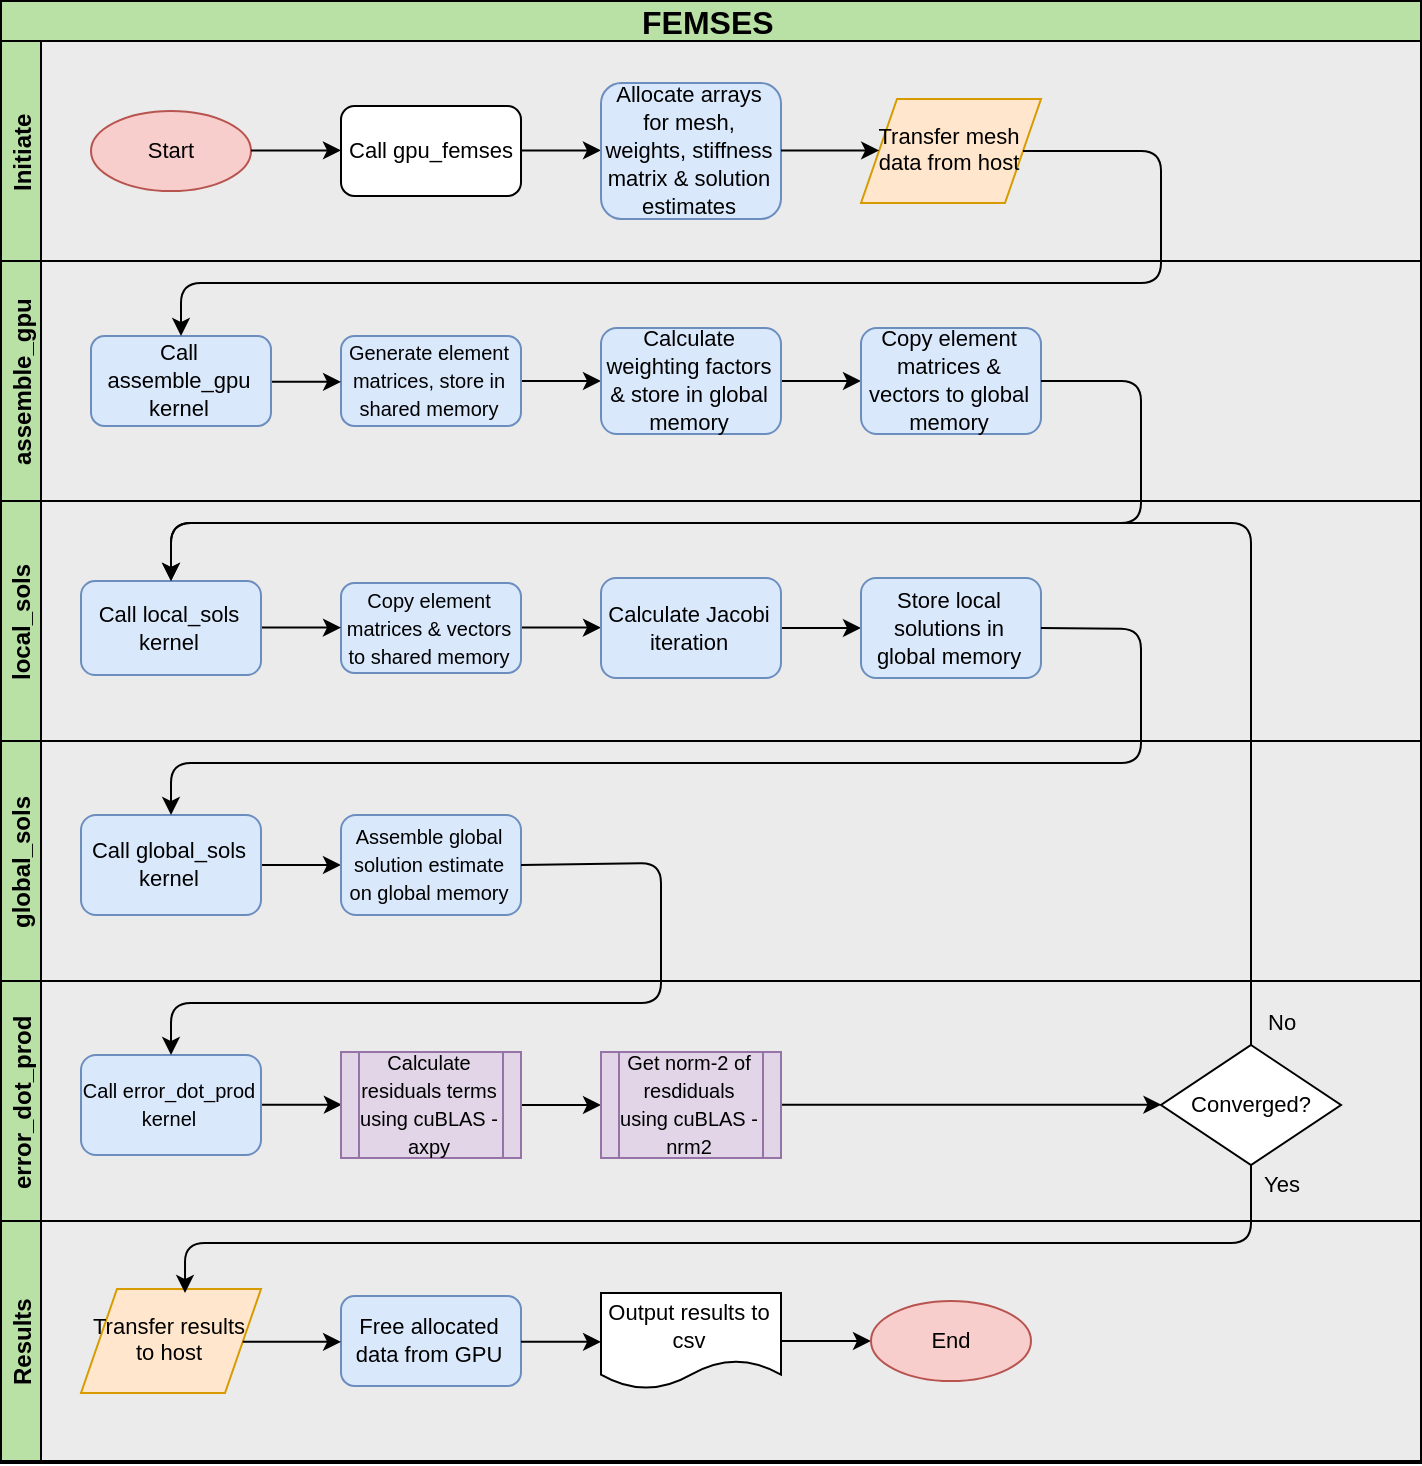
\includegraphics[width=0.9\linewidth]{Figures/femses_flow}
	\caption{Flowchart of FEMSES approach.}
	\label{fig:femsesflow}
\end{figure}

Figure~\ref{fig:femsesflow} shows a float chart of the FEMSES process when applied with CUDA code. Like before, the coloured steps are carried out by/on the GPU, the white are the host C++ functions. Unlike in Fernandez (CITE), the assembly of the element matrices is carried out on the GPU, and stored into global memory instead of being transferred by the host to device - this should show some speed-ups over the results seen. Just like in the standard FEM implementation, all the mesh creation operations are carried out on the host and transferred down, in this case excluding the sparsity scan as there is no global matrix ever assembled in this method. The kernels are divided up in quite a logical manner, but this is simply due to synchronisation limitations on the CUDA cores. Everything that can be completed in a single kernel without needing a global synchronisation, is completed as such. Unfortunately, any point that needs global memory synchronisation, will require a kernel to terminate. This can be seen in the flow chart, where the element matrices are assembled and stored into global memory, and using these, local solutions are calculated using the Jacobi relaxation and stored into global memory. Following that, another kernel assembles the global solution, again writing back to global memory. Lastly, cuBLAS is called in order to calculate the 2-norm of the error and check for convergence. Clearly at each of these steps, global memory must synchronise and so there was no option but to write these all in separate kernels.

\subsubsection{Storage \& Memory Management}

The FEMSES approaches shares the exact same memory allocations as the standard GPU FEM approach does, when it comes to allocating for the mesh. The same five arrays must be allocated and transferred taking up an identical amount of bytes as Equation~\eqref{mem}. After this point though, the two differ. Clearly, since the aim of the FEMSES approach is to avoid generating a global stiffness matrix and stress vector, then there will be no need to allocate space for them. Instead rather, two arrays must be allocated, both containing all of the element matrices and element vectors, \texttt{Le},\texttt{be} - these will be of size $\texttt{num\_cells}\times\texttt{9}\times\texttt{sizeof(float)}$ and $\texttt{num\_cells}\times\texttt{3}\times\texttt{sizeof(float)}$. There must also be space allocated to store an array of all the local element solutions \texttt{ue}, for when they are written back from shared memory, which is the same size as \texttt{be}. Finally there must be memory allocated to store both previous and new global solution estimates in the iteration, \texttt{up\_gpu}, \texttt{un\_gpu}, and an array containing the denominator of all the weightings, \texttt{w}  as seen in Equation~\eqref{weight} - all three of these are size $\texttt{order}\times\texttt{sizeof(float)}$ each. In total then, the global memory needed to perform FEMSES is,
\begin{flalign}
	\texttt{mem\_alloc\_femses} = \texttt({26}\times\texttt{order) + 72}\times\texttt{num\_cells)}. &&
\end{flalign}

For transfers, all of the data that is allocated besides the mesh is calculated on the GPU, and only the resulting global solution needs to be transferred. Besides this, there is also one single float transferred at every iteration to check for convergence, of course this is not known a priori so for arguments sake, if there is \texttt{iter} iterations before convergence then the total data transferred is,
\begin{flalign}
	&\texttt{mem\_transf\_femses} = \texttt{(18}\times\texttt{order) + (12}\times\texttt{num\_cells) + (4}\times\texttt{iter)}. &&
\end{flalign}

\subsubsection{Kernels}

The FEMSES approach is divided up into four component kernels as seen in Figure~\ref{fig:femsesflow}:
\begin{enumerate}
	\item generate element matrices.
	\item calculate local element solutions.
	\item assemble global solution estimate.
	\item calculate 2-norm of error.
\end{enumerate}
In the cases of the first three kernels, the grid structure is identical to what was seen in the general FEM approach, allowing maximum use of shared memory and attempts to prevent thread divergence.

The first kernel, listed in Listing (REFERENCE), is called on to generate the element matrices. It uses the same device function as the main kernel in the alternate approach to generate the element matrices on shared memory. After this, it calls on a device function to calculate the weightings and save them onto global memory. Lastly it writes the element matrices and element vectors to the array in global memory and terminates the kernel.

The second kernel, evaluates the local solution estimates. Illustrated in Listing (REFERENCE), this has two main device functions: the first reads in the element matrices and element vectors from global to shared memory. The second device function is the key computational step of this approach, calculating the Jacobi iteration estimate, as seen in Equation~\eqref{jacobi}, to generate local solutions and writes these back to global memory.

The final purpose-written kernel in this method assembles the global solution array using the weightings. Seen in Listing (REFERENCE), there was in fact no need for extra device functions here simply due to the fact that it was a read/write operation and one line of calculation - an atomic addition did sufficiently here. Thankfully, due to the irregular memory access pattern the atomic add should not actually pose much bottleneck. In Fernandez (CITE), the residuals were also calculated in this kernel, which is believed to be an oversight or error since this will potentially cause a race  condition as there is no guarantee the entire global solution has been assembled until the kernel terminates.

The final calculation kernel here is utilising cuBLAS. The kernel uses two BLAS Level-1 operations, the first being the vector product, $y \leftarrow \alpha x + y$, or \texttt{cublasSaxpy}, to evaluate the residual vector and write it over $y$. The second operation evaluates the 2-norm of the residual, $e \leftarrow \sqrt{\langle r, r\rangle}$, or \texttt{cublasSnrm2}. The resulting error term is passed back to the device.

\subsubsection{Device Functions}

The first device function utilised in the FEMSES approach is actually code reuse from the standard approach. It takes the mesh as input, uses the same shared memory structure as Figure (REFERENCE), and generates the element matrices and vectors in parallel, writing them to shared memory. See Section~\ref{basicfem} for more details on this device function.

The next device function evaluates the weightings. This functions takes the cell indices and element matrices as input and calculates the denominator weighting seen in Equation~\eqref{weight}. In Fernandez (CITE), each node in each cell was assigned its own individual weighting value in an array. This would involve a global synchronisation (something they did not do) to ensure the denominator values were fully added up and to avoid a race condition. Instead, the weighting array was allocated as one value per node as opposed to three per cell. In this paper's approach, the denominator was the weight stored and this was simply used to divide the node's corresponding diagonal value in its element matrix later on. Of course this means an extra read from global memory but it avoids the need for a global synchronisation.

The key device function in the entire approach is the Jacobi iteration function. Listing (REFERENCE) details this. Taking the previous global solution estimate as an input, it reads this in as $u^{(\texttt{old})}$, as well as reading in the element matrices and element vectors. Each thread will calculate its own individual $u^{(\texttt{new})}$, this will be written back to global memory then, to be assembled into a new global solution estimate using the succeeding kernel.

There are also another couple of device functions not mentioned here or in the previous section but these are merely read/write functions or area calculations et cetera.

\clearpage
\chapter{Results}

\section{Test-bed Architecture}

The problem stated in Section~\ref{problem} was used to computationally test the topics discussed in this paper. In terms of test bed architecture, the timings were all conducted on a 3.4~Ghz Intel Core~i5-3570K. with 6~Mb cache and 4 cores along with 16~GB of DDR3 memory. For the GPU times, two cards were used: a Kepler architecture, Tesla~K40 clocking 745~Mhz-875~Mhz, carrying 15 SMs, each with 192 CUDA cores, it carries 12~GB of GDDR5 global memory clocking 1.5~GHz and a 288~GB/s bandwidth. The other card tested was the more modern, Turing architecture, RTX~2080 Super, clocking at 1.65~Ghz-1.815~Ghz, carrying 48 SMs, each with 64 CUDA cores, 8~GB of GDDR6 memory with a 496GB/s bandwidth. Both cards have 48~Kb of shared memory per block and 16~Kb of per thread memory available. Note also, due to the limitations of the most recent version of Nvidia's Visual Profiler tool, installed on the system mentioned, and also the removal of some of the counters from the Turing architecture, for profiling, a different system with an older version of NVVP and an older (CARD). Table~\ref{table:testbed} illustrates all the specifications for the setup.
\begin{table}
    \begin{center}
    \resizebox{\columnwidth}{!}{
    \begin{tabular}{C{8em}|C{4em}C{5em}C{4em}C{6em}C{7em}C{5em}C{5em}C{5em}@{}m{0pt}@{} }
        %\Xhline{3\arrayrulewidth}
        \hline
        GPU & Arch & Clock~Speed & SMs & CUDA~Cores & DRAM & Clock~Speed & Bandwidth & Shared &\\[1.35em]
        \hline
        Tesla~K40 & Kepler & 745~Mhz & 15 & 2880 & 12~GB~GDDR5 & 1.5~Ghz & 288~GB/s & 46~Kb &\\[1.15em]
        RTX~2080~Super & Turing & 1.65~Ghz & 48 & 3072 & 8~GB~GDDR6 & ?~Ghz & 496~GB/s & 46~Kb &\\[1.15em]
        OTHER~CARD & Kepler & 445~Mhz & 15 & 2880 & 12~GB GDDR5 & 1.5~Ghz & 288~GB/s & 46~Kb &\\[1.15em]
        %\Xhline{3\arrayrulewidth}
        \hline
    \end{tabular}}
    \caption{Testbed architecture.}
	\label{table:testbed}
	\end{center}
\end{table}
    
From a software perspective, all serial code was written in C++11 and compile using \texttt{gcc5.4.0} with \texttt{-O3} flag enabled. The \texttt{-std=c++11} flag was of course enabled to ensure that the correct version of C++ and the STL was being utilised. In order to take advantage of the linear solvers, the Intel's MKL 18.0.4 library also needed to be called compiled with the serial code. To enable this, the binary executable and library files needed to be appended to the \texttt{PATH} and \texttt{LD\_LIBRARY\_PATH} environment variables, this was done by either calling the correct modules, if available or manually appending by,
\begin{lstlisting}[language=bash, basicstyle=\small\ttfamily ]
export PATH=$PATH:/home/support/apps/intel/18.0.4/bin/
export LD_LIBRARY_PATH=$LD_LIBRARY_PATH:
	/home/support/apps/intel/18.0.4/mkl/lib/intel64/intel64/
\end{lstlisting}
. The list of flags then needed for the Make were as follows,
\begin{itemize}
	\item \texttt{-lm}
	\item \texttt{-lmkl\_intel\_lp64}
	\item \texttt{-lmkl\_sequential}
	\item \texttt{-lmkl\_core}.
\end{itemize}

For the GPU code, all of it was written in CUDA with the most recent 10.1 SDK. The code was compiled with \texttt{nvcc} and \texttt{-O3} flag enabled again. In the implementation, certain device functions are shared across different headers so the \texttt{--relocatable-device-code=true} flag had to be enabled. the last consideration for the setup is the CUDA SDK~10.1, and its libraries used for linear solutions and BLAS operations. To enable these, again the \texttt{PATH} and \texttt{LD\_LIBRARY\_PATH} environment variables had to be appended, in this instance by,
\begin{lstlisting}[language=bash, basicstyle=\small\ttfamily ]
export PATH=$PATH:/usr/local/cuda-10.1/bin
export LD_LIBRARY_PATH=$LD_LIBRARY_PATH:/usr/local/cuda-10.1/lib64
\end{lstlisting}
. The list of flags then needed:
\begin{itemize}
	\item \texttt{-lcusolver}
	\item \texttt{-lcusparse}
	\item \texttt{-lcublas}.
\end{itemize}

\section{Serial Code Profiling}

\section{GPU Performance}

\subsection{Standard FEM}

\subsection{FEMSES}

\subsection{Comparison of GPU Architectures}

\clearpage
\chapter{Conclusion}

\section{Final Remarks}

In this paper, a serial implementation of the FEM was completed to solve a generic PDE problem posed used C++11. The code was partitioned into three main sections, the mesh generation, assembling the global stiffness matrix, and solving the  linear system. The mesh generation and application of the FEM were written using classes and some of C++11 STL features. The linear solver for the global system was implemented using Intel's MKL solver libraries. This serial version of the FEM was written to work for both sparse and dense global stiffness matrices and the assembly portion came in two different variants, applying DSS and LAPACKE for the solving portion, respectively. A sparsity scanner had to be implemented as part of the Mesh class in order to a priori deduce the sparsity pattern of the resulting FEM, so as to be able to assemble the CSR matrix. This was done using graph theory logic and using STL's sets. Both implementations were profiled to deduce the most dominant kernel in the process and tested up to problem sizes of 40,000 unknowns for the dense case and 490,000 for the sparse. In all cases, the solver resulted in being by a long stretch the most computationally expensive kernel. The results of the code were compared against analytical solutions found in Wolfram Mathematica. The code was timed to see how much of an improvement was seen by applying a sparse solution over a dense and it was seen that Intel's DSS was extremely efficient, taking around 2000~ms to solve for 40,000 unknowns, compared to 500,000~ms for the dense. The sparse solver also saw far more impressive linear scaling compared to the dense solver's quadratic - indicating that the speed-ups would only grow as problem size got larger.

The FEM implementations were then investigated for potential scope for parallelisation an naive sparse and dense implementations were then ported onto CUDA code for running on Nvidia's GPUs. There were many considerations taken when performing the port, such as thread divergence, optimising shared memory usage and reducing over-synchronisation. The main CUDA code purpose-written was for optimising and parallelising the generation of the element matrices and assembly of the global stiffness matrices. The solvers, again, were taken from pre-existing libraries. For the naive CUDA implementation, three solver variants were used, taken from Nvidia's cuSPARSE and cuSOLVER - one which solves a CSR, one which converts from dense to CSR and solves, and finally a dense solver. These were tested and timed for various different problem sizes and block sizes against their corresponding serial versions. Overall, again for the CUDA version, the solvers were the most dominant kernel - in this case even more so, achieving up to 99.5\% computation time. Nvidia's CSR solver did not perform as well as Intel's DSS, showing actual slowdown, while the dense solver outperformed its serial version with speed-ups of around $50\times$. 

It was noted after the first prototype of the code that there was a large portion of thread register usage and so an optimisation strategy was implemented to reconfigure the proportion of on-chip memory allocated to registers or shared memory. This saw no difference to the solver times, but did see improvements in the generation of the element matrices and assembly of the global system steps. These both saw huge speed-ups over the serial code, with the element matrices seeing $5000\times$ and the assembly seeing $20000\times$ and $120000\times$ times for the sparse and dense cases, respectively. Other profiling was done such as timing allocation and transfer time to check if the scaling is as should be expected given the memory needed - which it was shown to be. Profiling was also done on NVVP to show a minimal effect of warps causing thread divergence, and the improvement in memory usage, as well as the main contributing stall factors and the load distribution.

The next step taken in this report was the write the novel FEM Single Element Solution (FEMSES) implementation - which removes the assembly step from the traditional FEM and applies a Jacobi relaxation scheme on the local element solutions instead. Again, careful considerations like above had taken when implementing the code in CUDA due to GPU limitations. The code was structured into four main constituent kernels, one to generate the element matrices and store them in global memory, one to apply the Jacobi iteration, one to assemble the global solution estimate and finally one to evaluate the 2-norm of the error in the current iteration. The last kernel made use of pre-existing cuBLAS functions to calculate the error. Again, the code was timed and profiled to deduce performance factors. Overall the FEMSES approach didn't see the same speeds demonstrated in Fernandez~\cite{femses}. It did outperform and scale better than the dense serial case and also had an positive trend for against the naive GPU dense case. In both sparse cases, however, it was outperformed. This was down to poor convergence more so than poorly performing code, as seen in the reasonably good timings when the problem size is small and the convergence rate low. It is suspected this was due to the choice of PDE causing propagation from only two boundaries but this has yet to be tested. This FEMSES implementation was also profiled using NVVP showing good load balance, no thread divergence and a mixed collection of reasons for latencies.

The final thing tested, within the time constraints of this report, was comparing the speeds of the two different cards in the test-bed architecture. All of the previous timings were completed on a Tesla~K40 as the newer RTX~2080 Super had yet to be installed. Once this was, however, the two were compared for timings. The Tesla was outperformed in most of the tests barring the FEMSES implementation. This is potentially down to the fact that the newer cards might have optimised Nvidia's existing libraries better, whereas the FEMSES approach was written on a Tesla and solely tested prior to that on the Tesla and so wasn't written to be optimised on the RTX~2080 Super. That being said, there was some quite positive speed-ups, in some cases reaching double digits.

Concluding then, in investigations in this paper saw a mixed collection of results. In the instances of dense cases, the overall results were quite positive and all showed very positive scaling. For the sparse cases, however, the dominance of the solver portion of the FEM overshadowed the speed-ups seen in the other steps due to the blistering performance of Intel's DSS dominating Nvidia's solver and the FEMSES solver. 

\section{Future Work}

\begin{figure}
	\centering
	\begin{subfigure}{0.35\linewidth}
		\centering
		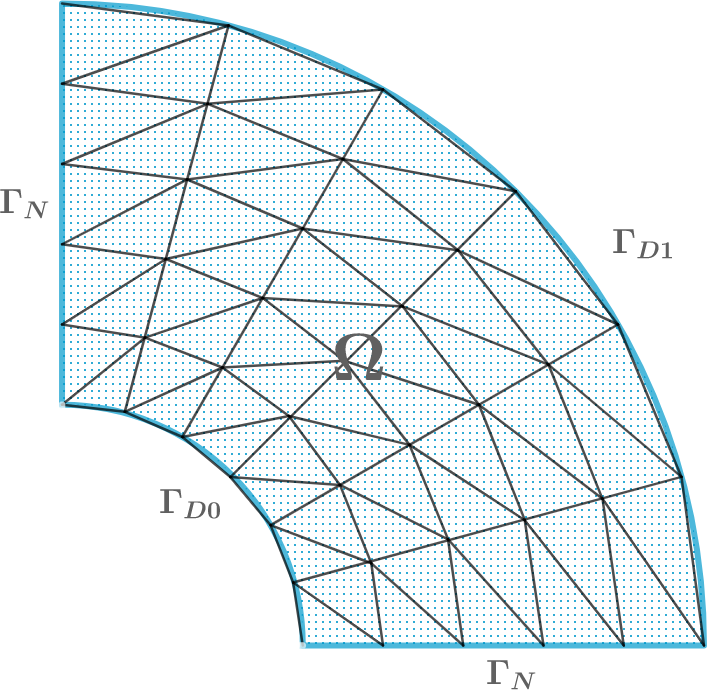
\includegraphics[width = \linewidth]{Figures/annulus}
		\caption{Annulus domain of initially proposed PDE.}
		\label{fig:annul_dom}
	\end{subfigure}\hfill
	\begin{subfigure}{0.53\linewidth}
		\centering
		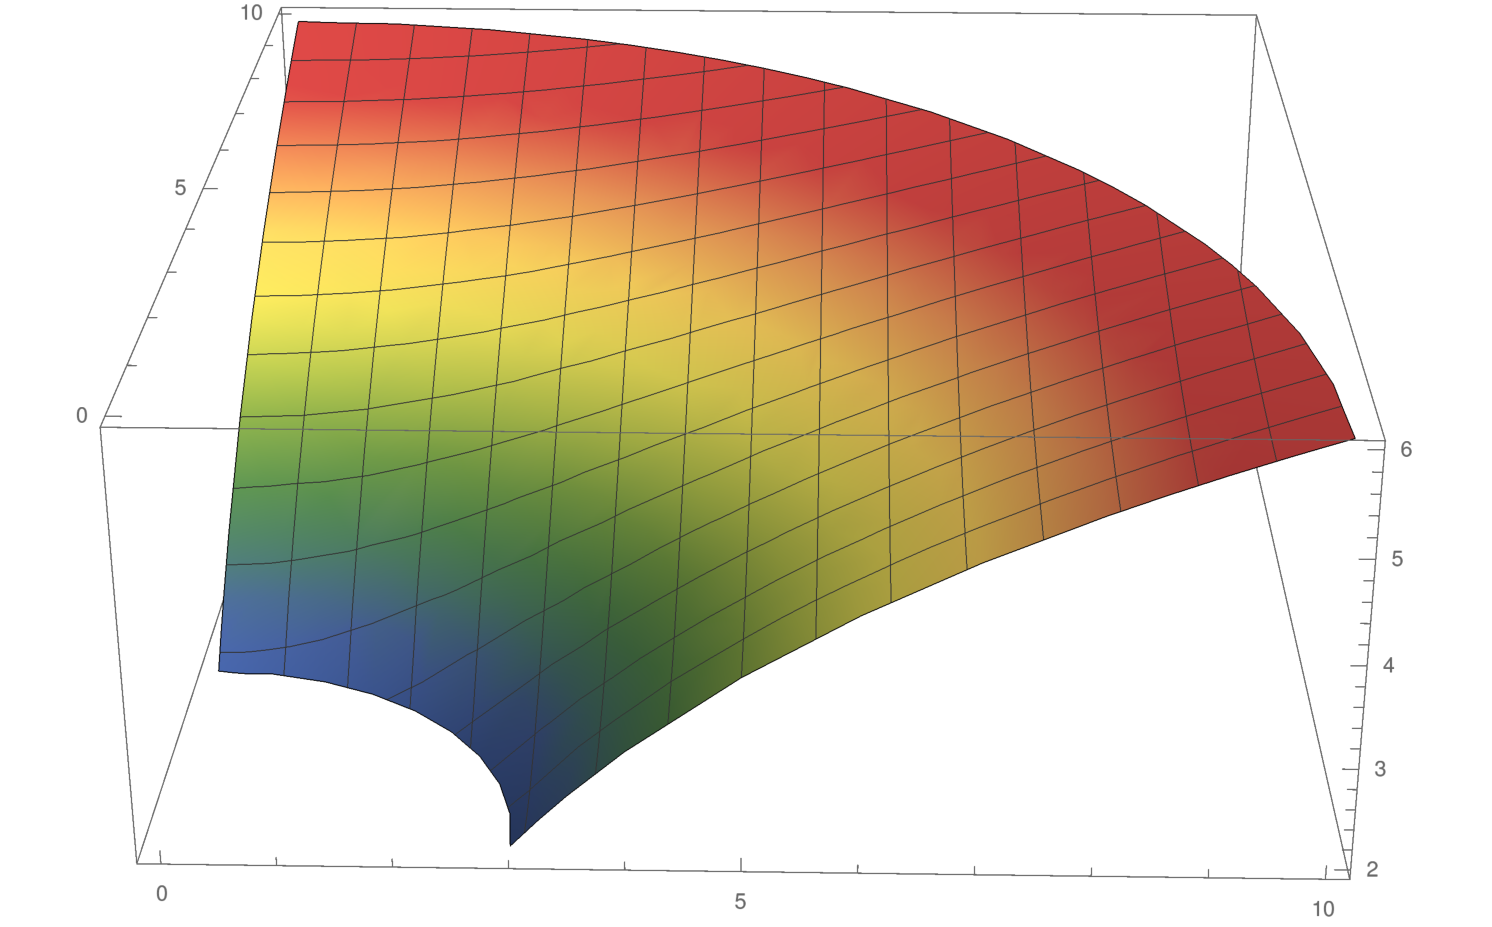
\includegraphics[width=\linewidth]{Figures/annul}
		\caption{Solution from Mathematica of initially proposed PDE..}
		\label{fig:annul_sols}
	\end{subfigure}
	\caption{Domain and solution of initially proposed PDE.}
	\label{fig:init_pde}
\end{figure}

There are still many things to consider at the end of this report - almost endless in reality when it comes to GPU programming. However, there are a few points that would be rather interesting to further investigate if time was permitting. The first one of note is, when coding the serial implementation, the initial plan was to use a PDE with a relatively unusual mesh, such as the one seen in Figure~\ref{fig:init_pde} - since robustness in mesh shape is one of the biggest benefits of choosing the FEM over the finite difference. There wasn't an aim to pick an overly complicated PDE since the purpose of the paper was to test performances, but an interesting mesh like an annulus would have done nicely. It was noted, however, that when using the formulae in Section~\ref{problem}, that in Davies~\cite{davies}, there appeared to have been some assumption made that wasn't clear, that these only work when the cells are all of equal size. It would be a good expansion on the paper to add some numerical integration to evaluate the element matrices instead of those formulae - which would solve the issue of the varying cell size causing problems. The code for the annulus transformation is still in the implementation for future tests. It would even be a nice possibility to add dynamic parallelism to perform the numerical integration on the CUDA implementations.

Another point of potential further study, and probably the most important to this paper, in reality, is to deduce the reason behind the poor rate of convergence for FEMSES compared to in its original literature. The thinking at the time of writing is, since the PDE chosen was a Laplace, which has a sparse RHS vector barring boundary condition enforcements, the propagation from the boundary conditions could be a large factor in the rate of convergence. In this paper, only two of the boundaries were non-homogeneous, resulting in propagation from only two directions. Without yet, of course, having the chance to test this, if a PDE were chosen which has a domain causing it to propagate from more directions, like the one in the FEMSES paper, this might show improved rates of convergence.

If this investigation into the convergence proved fruitful, a next step would be to implement the other FEM GPU implementation discussed, the domain decomposition and multigrid techniques. It would be interesting to see how a fully functioning FEMSES would compare to a method as efficient as multigrid. On top of this, furthering on from not only improving the naive implementation, but with a working FEMSES, an interesting further development would also be to use a different iterative relaxation to Jacobi - which traditionally has poor convergence anyway. This could prove tricky however, given that the input vector and output vector for this semi-Jacobi method are not actually the same, but one rather is a global solution portion and one the local solution. Some consideration would need to go into how to port this even to something like Gauss-Seidel where the most recent update is needed - which would involve the assembly of the global solution estimate at each row in the given iteration.

One final last point for further study that would be important to address is the dominance of the linear solvers - in both computation time and also memory allocation. The choice to use pre-existing solver libraries was done both for convenience and for expected efficiency given the amount of optimisations put into them. However, most of the libraries used direct solvers. These are not optimal for sparse matrices and also, when running took orders more memory. For a case where the amount of memory allocated to the GPU was 208~Mb for the mesh and matrices, Nvidia's cuSOLVER allocated 10.8~Gb to perform its linear solver - this would not happen for iterative methods. It would be good to see how something like the preconditioned Conjugate Gradient method would perform against its serial counterpart.


%%%%%%%%%%%%%%%%%%%%%%%%%%%%%%%%%%%%%%%%%%%%%%%%%%%%%%%%%%%%%
%BIBLIOGRAPHY
%%%%%%%%%%%%%%%%%%%%%%%%%%%%%%%%%%%%%%%%%%%%%%%%%%%%%%%%%%%%%

\clearpage
\renewcommand*{\thesection}{}\textbf{}

\bibliographystyle{apacite}
\bibliography{Bibliography.bib}


%%%%%%%%%%%%%%%%%%%%%%%%%%%%%%%%%%%%%%%%%%%%%%%%%%%%%%%%%%%%%
%APPENDICES
%%%%%%%%%%%%%%%%%%%%%%%%%%%%%%%%%%%%%%%%%%%%%%%%%%%%%%%%%%%%%

\appendix
\renewcommand*{\thesection}{\Alph{section}}\textbf{}

\begin{appendices}
\clearpage
\chapter{Appendix}
\label{app:A}
...
\end{appendices}


\end{document}